\documentclass[twoside]{book}

% Packages required by doxygen
\usepackage{fixltx2e}
\usepackage{calc}
\usepackage{doxygen}
\usepackage[export]{adjustbox} % also loads graphicx
\usepackage{graphicx}
\usepackage[utf8]{inputenc}
\usepackage{makeidx}
\usepackage{multicol}
\usepackage{multirow}
\PassOptionsToPackage{warn}{textcomp}
\usepackage{textcomp}
\usepackage[nointegrals]{wasysym}
\usepackage[table]{xcolor}

% Font selection
\usepackage[T1]{fontenc}
\usepackage[scaled=.90]{helvet}
\usepackage{courier}
\usepackage{amssymb}
\usepackage{sectsty}
\renewcommand{\familydefault}{\sfdefault}
\allsectionsfont{%
  \fontseries{bc}\selectfont%
  \color{darkgray}%
}
\renewcommand{\DoxyLabelFont}{%
  \fontseries{bc}\selectfont%
  \color{darkgray}%
}
\newcommand{\+}{\discretionary{\mbox{\scriptsize$\hookleftarrow$}}{}{}}

% Page & text layout
\usepackage{geometry}
\geometry{%
  a4paper,%
  top=2.5cm,%
  bottom=2.5cm,%
  left=2.5cm,%
  right=2.5cm%
}
\tolerance=750
\hfuzz=15pt
\hbadness=750
\setlength{\emergencystretch}{15pt}
\setlength{\parindent}{0cm}
\setlength{\parskip}{0.2cm}
\makeatletter
\renewcommand{\paragraph}{%
  \@startsection{paragraph}{4}{0ex}{-1.0ex}{1.0ex}{%
    \normalfont\normalsize\bfseries\SS@parafont%
  }%
}
\renewcommand{\subparagraph}{%
  \@startsection{subparagraph}{5}{0ex}{-1.0ex}{1.0ex}{%
    \normalfont\normalsize\bfseries\SS@subparafont%
  }%
}
\makeatother

% Headers & footers
\usepackage{fancyhdr}
\pagestyle{fancyplain}
\fancyhead[LE]{\fancyplain{}{\bfseries\thepage}}
\fancyhead[CE]{\fancyplain{}{}}
\fancyhead[RE]{\fancyplain{}{\bfseries\leftmark}}
\fancyhead[LO]{\fancyplain{}{\bfseries\rightmark}}
\fancyhead[CO]{\fancyplain{}{}}
\fancyhead[RO]{\fancyplain{}{\bfseries\thepage}}
\fancyfoot[LE]{\fancyplain{}{}}
\fancyfoot[CE]{\fancyplain{}{}}
\fancyfoot[RE]{\fancyplain{}{\bfseries\scriptsize Generated on Tue Jul 7 2015 15\+:12\+:35 for ht\textquotesingle{}s Scheme Intepreter by Doxygen }}
\fancyfoot[LO]{\fancyplain{}{\bfseries\scriptsize Generated on Tue Jul 7 2015 15\+:12\+:35 for ht\textquotesingle{}s Scheme Intepreter by Doxygen }}
\fancyfoot[CO]{\fancyplain{}{}}
\fancyfoot[RO]{\fancyplain{}{}}
\renewcommand{\footrulewidth}{0.4pt}
\renewcommand{\chaptermark}[1]{%
  \markboth{#1}{}%
}
\renewcommand{\sectionmark}[1]{%
  \markright{\thesection\ #1}%
}

% Indices & bibliography
\usepackage{natbib}
\usepackage[titles]{tocloft}
\setcounter{tocdepth}{3}
\setcounter{secnumdepth}{5}
\makeindex

% Hyperlinks (required, but should be loaded last)
\usepackage{ifpdf}
\ifpdf
  \usepackage[pdftex,pagebackref=true]{hyperref}
\else
  \usepackage[ps2pdf,pagebackref=true]{hyperref}
\fi
\hypersetup{%
  colorlinks=true,%
  linkcolor=blue,%
  citecolor=blue,%
  unicode%
}

% Custom commands
\newcommand{\clearemptydoublepage}{%
  \newpage{\pagestyle{empty}\cleardoublepage}%
}


%===== C O N T E N T S =====

\begin{document}

% Titlepage & ToC
\hypersetup{pageanchor=false,
             bookmarks=true,
             bookmarksnumbered=true,
             pdfencoding=unicode
            }
\pagenumbering{roman}
\begin{titlepage}
\vspace*{7cm}
\begin{center}%
{\Large ht\textquotesingle{}s Scheme Intepreter \\[1ex]\large 1.\+0 }\\
\vspace*{1cm}
{\large Generated by Doxygen 1.8.9.1}\\
\vspace*{0.5cm}
{\small Tue Jul 7 2015 15:12:35}\\
\end{center}
\end{titlepage}
\clearemptydoublepage
\tableofcontents
\clearemptydoublepage
\pagenumbering{arabic}
\hypersetup{pageanchor=true}

%--- Begin generated contents ---
\chapter{ht\+Scheme}
\label{md__r_e_a_d_m_e}
\hypertarget{md__r_e_a_d_m_e}{}
\#ht\+Scheme A structured and plugin-\/based scheme interpreter implementation.

\subsection*{How to use}

\subsubsection*{Prerequisites}


\begin{DoxyItemize}
\item A modern C++ compiler supporting c++11 feature. (gcc4.\+9.\+2, gcc5.\+1, clang3.\+6 have been tested on Linux)
\item G\+N\+U Make (Make v4.\+0 has been tested on Linux)
\end{DoxyItemize}

\subsubsection*{Make}

Enter the {\ttfamily scheme} directory and run the following commands to generate various targets\+:

\begin{TabularC}{2}
\hline
\rowcolor{lightgray}\PBS\centering {\bf {\bfseries Command} }&\PBS\centering {\bf {\bfseries Function}  }\\\cline{1-2}
\PBS\centering {\ttfamily make}={\ttfamily make all} &\PBS\centering Call everything below except {\ttfamily dep} and {\ttfamily clean} \\\cline{1-2}
\PBS\centering {\ttfamily make cli} &\PBS\centering Generate {\ttfamily cli} (the command-\/line interpreter frontend) \\\cline{1-2}
\PBS\centering {\ttfamily make dep} &\PBS\centering Generate {\ttfamily \hyperlink{dep_8d}{dep.\+d}} which contains the dependencies of files \\\cline{1-2}
\PBS\centering {\ttfamily make clean} &\PBS\centering Remove all files generated by {\ttfamily make} \\\cline{1-2}
\PBS\centering {\ttfamily make preprocessortest}&\PBS\centering Generate {\ttfamily preprocessortest} \\\cline{1-2}
\PBS\centering {\ttfamily make tokenizertest} &\PBS\centering Generate {\ttfamily tokenizertest} \\\cline{1-2}
\PBS\centering {\ttfamily make asttest} &\PBS\centering Generate {\ttfamily asttest} \\\cline{1-2}
\PBS\centering {\ttfamily make parserstest} &\PBS\centering Generate {\ttfamily parserstest} \\\cline{1-2}
\PBS\centering {\ttfamily make biginttest} &\PBS\centering Generate {\ttfamily biginttest} \\\cline{1-2}
\PBS\centering {\ttfamily make rationaltypetest}&\PBS\centering Generate {\ttfamily rationaltypetest} \\\cline{1-2}
\end{TabularC}
You may notice that the compilation is rather slow, therefore you can add {\ttfamily -\/j4} to {\ttfamily make} command in order to parallel the compilation with four threads.

\subsection*{How to develop with ht\+Scheme}

ht\+Scheme has been designed as an extensible architecture of scheme-\/like languages, thus new types of tokens as well as parsers could be easily added into this program.

\subsubsection*{Brief introduction to files}

\paragraph*{\hyperlink{preprocessor_8hpp}{preprocessor.\+hpp}/cpp}

```cpp class \hyperlink{class_scheme_unit}{Scheme\+Unit} \{ public\+: \hyperlink{class_scheme_unit}{Scheme\+Unit(std\+::istream\& scheme\+Stream)}; std\+::vector$<$std\+::string$>$ lines; void preprocess(std\+::istream\& scheme\+Stream); \}; ``{\ttfamily  Accept a}std\+::istream$<$tt$>$as the parameter, then read lines from it untilscheme\+Stream.\+eof(){\ttfamily and remove the comments with the result stored in}lines`.

\paragraph*{\hyperlink{tokenizer_8hpp}{tokenizer.\+hpp}/cpp}

```cpp class \hyperlink{class_tokenizer}{Tokenizer} \{ public\+: \hyperlink{class_tokenizer}{Tokenizer(const std\+::vector$<$std\+::string$>$\& lines)}; void split(const std\+::vector$<$std\+::string$>$\& lines); void parse(const std\+::list$<$std\+::string$>$\& raw\+Tokens); std\+::list$<$std\+::string$>$ raw\+Tokens; std\+::list$<$\+Token$>$ tokens; bool complete; \}; ``{\ttfamily  Accept lines of program, Then}\hyperlink{class_tokenizer_a2a6c04ea8c784f66bebcb6df7073769c}{Tokenizer\+::\+Tokenizer$<$tt$>$}will call\hyperlink{class_tokenizer}{Tokenizer}\+:split{\ttfamily and}Tokernizer\+::parse` in order.

{\ttfamily \hyperlink{class_tokenizer_a8bd8a4eb5df764f6128028daa0e9044b}{Tokenizer\+::split}} splits {\ttfamily lines} into several small string pieces stored in {\ttfamily \hyperlink{class_tokenizer_a89707ad3a758fc9ec58f00d92d5fc622}{Tokenizer\+::raw\+Tokens}}. For example, {\ttfamily (string-\/ith \char`\"{}123 34\char`\"{} 2)} will be split into ``` ( string-\/ith \char`\"{}123 34\char`\"{} 2 ) ```

{\ttfamily \hyperlink{class_tokenizer_ae928efe72c00908a3529747b4cfd01d5}{Tokenizer\+::parse}} convert {\ttfamily \hyperlink{class_tokenizer_a89707ad3a758fc9ec58f00d92d5fc622}{Tokenizer\+::raw\+Tokens}} to {\ttfamily \hyperlink{class_tokenizer_ae547093dbd03b3e70373147e4669d9fa}{Tokenizer\+::tokens}}.

{\ttfamily \hyperlink{struct_token}{Token}} is defined as followed in {\ttfamily \hyperlink{types_2all_8hpp}{types/all.\+hpp}}\+: ```cpp struct \hyperlink{struct_token}{Token} \{ Token\+Type token\+Type; //enum Token\+Type \{Op\+Plus, ...\} Info\+Types info; //typedef boost\+::variant$<$\+Info\+Type1, ...$>$ Info\+Types \}; ```

There is an extra variable {\ttfamily \hyperlink{class_tokenizer_a330a4cce0cbf3ebfbe601d97022d1ed4}{Tokenizer\+::complete}} in this class, which represents whether there is no incomplete brackets or quotaion marks. This could be useful in building command-\/line interpreter. {\ttfamily \hyperlink{class_tokenizer_a330a4cce0cbf3ebfbe601d97022d1ed4}{Tokenizer\+::complete}} can be set by both {\ttfamily \hyperlink{class_tokenizer_a8bd8a4eb5df764f6128028daa0e9044b}{Tokenizer\+::split}} and {\ttfamily \hyperlink{class_tokenizer_ae928efe72c00908a3529747b4cfd01d5}{Tokenizer\+::parse}}.

\paragraph*{\hyperlink{ast_8hpp}{ast.\+hpp}/cpp}

```cpp class \hyperlink{class_a_s_t}{A\+S\+T} \{ public\+: \hyperlink{struct_a_s_t_node}{A\+S\+T\+Node} ast\+Head; void build\+A\+S\+T(const std\+::list$<$\+Token$>$ \&tokens); \hyperlink{class_a_s_t}{A\+S\+T} (const std\+::list$<$\+Token$>$ \&tokens); \hyperlink{class_a_s_t}{A\+S\+T()}; friend std\+::ostream\& operator $<$$<$ (std\+::ostream\& o, const \hyperlink{class_a_s_t}{A\+S\+T}\& ast); \}; ``{\ttfamily  Build an \hyperlink{class_a_s_t}{A\+S\+T} which could be accessed through}\hyperlink{class_a_s_t_a4f9b6d3be381682515e1e51c176b1c21}{A\+S\+T.\+ast\+Head$<$tt$>$}withstd\+::list$<$\+Token$>$`.

Here is the definition of {\ttfamily \hyperlink{struct_a_s_t_node}{A\+S\+T\+Node}}\+: ```cpp struct \hyperlink{struct_a_s_t_node}{A\+S\+T\+Node} \{ Node\+Type type; //enum Node\+Type \{Bracket, Simple\}; \hyperlink{struct_token}{Token} token; A\+S\+T\+Node$\ast$ parent; std\+::list$<$\+A\+S\+T\+Node$\ast$$>$ ch;

A\+S\+T\+Node$\ast$ add(const A\+S\+T\+Node\& node); //ch.push\+\_\+back(new A\+S\+T\+Node(node)) void remove(); //\+Recursively remove all its children then clear ch \}; ```

For example, {\ttfamily (+ 2.\+7 (-\/ 5.\+6 2.\+1) 3)} will be converted to the following \hyperlink{class_a_s_t}{A\+S\+T}\+: ``` Type\+:0 \hyperlink{struct_token_a4c338f6ca199f4a8575e877d36d03a06}{Token.\+info}\+:0 Token\+Type\+:0 //ast\+Head +-\/---Type\+:Bracket \hyperlink{struct_token_a4c338f6ca199f4a8575e877d36d03a06}{Token.\+info}\+:0 Token\+Type\+:0 +---Type\+:Simple \hyperlink{struct_token_a4c338f6ca199f4a8575e877d36d03a06}{Token.\+info}\+:0 Token\+Type\+:Op\+Plus $\vert$---Type\+:Simple \hyperlink{struct_token_a4c338f6ca199f4a8575e877d36d03a06}{Token.\+info}\+:2.\+7 Token\+Type\+:Float $\vert$---Type\+:Bracket \hyperlink{struct_token_a4c338f6ca199f4a8575e877d36d03a06}{Token.\+info}\+:0 Token\+Type\+:0 $\vert$ +---Type\+:Simple \hyperlink{struct_token_a4c338f6ca199f4a8575e877d36d03a06}{Token.\+info}\+:0 Token\+Type\+:Op\+Minus $\vert$ $\vert$---Type\+:Simple \hyperlink{struct_token_a4c338f6ca199f4a8575e877d36d03a06}{Token.\+info}\+:5.\+6 Token\+Type\+:Float $\vert$ $\vert$---Type\+:Simple \hyperlink{struct_token_a4c338f6ca199f4a8575e877d36d03a06}{Token.\+info}\+:2.\+1 Token\+Type\+:Float $\vert$---Type\+:Simple \hyperlink{struct_token_a4c338f6ca199f4a8575e877d36d03a06}{Token.\+info}\+:3 Token\+Type\+:Float ```

\paragraph*{\hyperlink{parsers_8hpp}{parsers.\+hpp}}

The main part of {\ttfamily \hyperlink{parsers_8hpp}{parsers.\+hpp}} is in {\ttfamily \hyperlink{parsers_2all_8hpp}{parsers/all.\+hpp}}

```cpp class \hyperlink{class_parsers_helper}{Parsers\+Helper} \{ \hyperlink{class_parsers_helper}{Parsers\+Helper()}; void parse(\+A\+S\+T\+Node\& astnode); \}; ``{\ttfamily  Provide a reference of}\hyperlink{struct_a_s_t_node}{A\+S\+T\+Node}{\ttfamily to an instance of}\hyperlink{class_parsers_helper_a21ce6213ee29e0459dd655c6803db00b}{Parsers\+Helper\+::parse$<$tt$>$}, then\hyperlink{class_parsers_helper}{Parsers\+Helper}{\ttfamily will call according}xxx\+A\+S\+T\+Parser\+::parse(\+A\+S\+T\+Node\& parent, Parsers\+Helper\& helper){\ttfamily to recursively calculate the result of a subtree of \hyperlink{class_a_s_t}{A\+S\+T} with its root as}astnode{\ttfamily . After}\hyperlink{class_parsers_helper_a21ce6213ee29e0459dd655c6803db00b}{Parsers\+Helper\+::parse$<$tt$>$},astnode.\+type$<$tt$>$will becomeSimple{\ttfamily . If}astnode{\ttfamily is already a}Simple` node, nothing will be done.

The parsed version of the above \hyperlink{class_a_s_t}{A\+S\+T} is (by calling {\ttfamily parse( $\ast$$\ast$ast.head\+Node.\+ch.\+begin() )}\+: ``` Type\+:1 \hyperlink{struct_token_a4c338f6ca199f4a8575e877d36d03a06}{Token.\+info}\+:0 Token\+Type\+:0 //head\+Node +-\/---Type\+:Simple \hyperlink{struct_token_a4c338f6ca199f4a8575e877d36d03a06}{Token.\+info}\+:9.\+2 Token\+Type\+:Float ```

{\bfseries Warning} --D\+O N\+O\+T-- directly call {\ttfamily helper.\+parse($\ast$ch\mbox{[}xx\mbox{]})} in {\ttfamily xxx\+A\+S\+T\+Parser\+::parse(\+A\+S\+T\+Node\& parent, Parsers\+Helper\& helper)} ! Instead, you should copy construct a new {\ttfamily \hyperlink{class_parsers_helper}{Parsers\+Helper}} to parse its children.

\subsubsection*{Add your own \hyperlink{struct_token}{Token} Parser}

In this section, we will try to add a new {\ttfamily Rational} type of token.

\paragraph*{Step1\+: Register the Rational Type}

Open {\ttfamily \hyperlink{types_2arch_8hpp}{types/arch.\+hpp}}, add {\ttfamily Rational} to {\ttfamily enum Token\+Type\{ ... , Rational \}}

\paragraph*{Step2\+: Register the Rational Parser}


\begin{DoxyItemize}
\item Open {\ttfamily \hyperlink{types_2all_8hpp}{types/all.\+hpp}}, add {\ttfamily Rational\+Parser} to {\ttfamily \#define P\+A\+R\+S\+E\+R\+S\+\_\+\+T\+U\+P\+L\+E (..., Rational\+Parser)}
\item {\ttfamily \#include \char`\"{}rational.\+hpp\char`\"{}}
\end{DoxyItemize}

\paragraph*{Step3\+: Write the Header}


\begin{DoxyItemize}
\item Create {\ttfamily \hyperlink{rational_8hpp}{types/rational.\+hpp}}, then include your declaration of your {\ttfamily \hyperlink{class_rational_type}{Rational\+Type}} and {\ttfamily \char`\"{}arch.\+hpp\char`\"{}}
\item Use the macro in {\ttfamily arch.\+hpp} to generate the declaration of your {\ttfamily Rational\+Parser} \+: ``` \hyperlink{types_2arch_8hpp_a669f5b829a7373f20602e4c063e01d99}{P\+A\+R\+S\+E\+R\+\_\+\+D\+E\+C\+L\+A\+R\+A\+T\+I\+O\+N(\+Rational\+Parser, Rational, Rational\+Type)} ```
\end{DoxyItemize}

\paragraph*{Step4\+: Implement the Parser}


\begin{DoxyItemize}
\item Create {\ttfamily \hyperlink{rational_8cpp}{types/rational.\+cpp}}, then {\ttfamily \#include \char`\"{}rational.\+hpp\char`\"{}} and implement your {\ttfamily \hyperlink{class_rational_type}{Rational\+Type}} in it.
\item Implement {\ttfamily bool Rational\+Parser\+::judge(const std\+::string\& token)} which returns whether a token is a rational token and {\ttfamily Rational\+Parser\+::\+Info\+Type Rational\+Parser\+::get(const std\+::string\& token)} which converts the token to {\ttfamily Rational\+Parser\+::\+Info\+Type}(aka {\ttfamily \hyperlink{class_rational_type}{Rational\+Type}})
\item {\ttfamily const Token\+Type Rational\+Parser\+::type = Rational;} 
\end{DoxyItemize}
\chapter{Class Index}
\section{Class List}
Here are the classes, structs, unions and interfaces with brief descriptions\+:\begin{DoxyCompactList}
\item\contentsline{section}{\hyperlink{class_big_int}{Big\+Int} }{\pageref{class_big_int}}{}
\item\contentsline{section}{\hyperlink{struct_parenthesis_info}{Parenthesis\+Info} }{\pageref{struct_parenthesis_info}}{}
\item\contentsline{section}{\hyperlink{class_rational_type}{Rational\+Type} }{\pageref{class_rational_type}}{}
\item\contentsline{section}{\hyperlink{class_scheme_unit}{Scheme\+Unit} }{\pageref{class_scheme_unit}}{}
\item\contentsline{section}{\hyperlink{class_tokenizer}{Tokenizer} }{\pageref{class_tokenizer}}{}
\end{DoxyCompactList}

\chapter{File Index}
\section{File List}
Here is a list of all files with brief descriptions\+:\begin{DoxyCompactList}
\item\contentsline{section}{\hyperlink{_8ycm__extra__conf_8py}{.\+ycm\+\_\+extra\+\_\+conf.\+py} }{\pageref{_8ycm__extra__conf_8py}}{}
\item\contentsline{section}{\hyperlink{preprocessor_8cpp}{preprocessor.\+cpp} }{\pageref{preprocessor_8cpp}}{}
\item\contentsline{section}{\hyperlink{preprocessor_8hpp}{preprocessor.\+hpp} }{\pageref{preprocessor_8hpp}}{}
\item\contentsline{section}{\hyperlink{tokenizer_8cpp}{tokenizer.\+cpp} }{\pageref{tokenizer_8cpp}}{}
\item\contentsline{section}{\hyperlink{tokenizer_8hpp}{tokenizer.\+hpp} }{\pageref{tokenizer_8hpp}}{}
\item\contentsline{section}{\hyperlink{types_8hpp}{types.\+hpp} }{\pageref{types_8hpp}}{}
\item\contentsline{section}{test/\hyperlink{biginttest_8cpp}{biginttest.\+cpp} }{\pageref{biginttest_8cpp}}{}
\item\contentsline{section}{test/\hyperlink{preprocessortest_8cpp}{preprocessortest.\+cpp} }{\pageref{preprocessortest_8cpp}}{}
\item\contentsline{section}{test/\hyperlink{tokenizertest_8cpp}{tokenizertest.\+cpp} }{\pageref{tokenizertest_8cpp}}{}
\item\contentsline{section}{types/\hyperlink{all_8hpp}{all.\+hpp} }{\pageref{all_8hpp}}{}
\item\contentsline{section}{types/\hyperlink{arch_8hpp}{arch.\+hpp} }{\pageref{arch_8hpp}}{}
\item\contentsline{section}{types/\hyperlink{boolean_8hpp}{boolean.\+hpp} }{\pageref{boolean_8hpp}}{}
\item\contentsline{section}{types/\hyperlink{float_8cpp}{float.\+cpp} }{\pageref{float_8cpp}}{}
\item\contentsline{section}{types/\hyperlink{float_8hpp}{float.\+hpp} }{\pageref{float_8hpp}}{}
\item\contentsline{section}{types/\hyperlink{ops_8hpp}{ops.\+hpp} }{\pageref{ops_8hpp}}{}
\item\contentsline{section}{types/\hyperlink{parenthesis_8hpp}{parenthesis.\+hpp} }{\pageref{parenthesis_8hpp}}{}
\item\contentsline{section}{types/\hyperlink{rational_8hpp}{rational.\+hpp} }{\pageref{rational_8hpp}}{}
\item\contentsline{section}{types/\hyperlink{string_8hpp}{string.\+hpp} }{\pageref{string_8hpp}}{}
\item\contentsline{section}{utility/\hyperlink{bigint_8cpp}{bigint.\+cpp} }{\pageref{bigint_8cpp}}{}
\item\contentsline{section}{utility/\hyperlink{bigint_8hpp}{bigint.\+hpp} }{\pageref{bigint_8hpp}}{}
\item\contentsline{section}{utility/\hyperlink{strutility_8hpp}{strutility.\+hpp} }{\pageref{strutility_8hpp}}{}
\end{DoxyCompactList}

\chapter{Class Documentation}
\hypertarget{class_big_int}{}\section{Big\+Int Class Reference}
\label{class_big_int}\index{Big\+Int@{Big\+Int}}


{\ttfamily \#include $<$bigint.\+hpp$>$}

\subsection*{Public Member Functions}
\begin{DoxyCompactItemize}
\item 
\hyperlink{class_big_int_a4421e6c1883874512f1b04543dafc64a}{Big\+Int} (long long num)
\item 
\hyperlink{class_big_int_abe13ffcbf871ddb97365a73120ca0b6f}{Big\+Int} (const std\+::string \&\hyperlink{preprocessortest_8cpp_a10d1ea193b80aa2128e080646057d11c}{s})
\item 
\hyperlink{class_big_int_af677021c0987fc2a48da06837ed29c58}{Big\+Int} ()
\item 
\hyperlink{class_big_int}{Big\+Int} \& \hyperlink{class_big_int_a43652944006a9ace4fa3d8e1c0ed3213}{assign} (long long num)
\item 
\hyperlink{class_big_int}{Big\+Int} \& \hyperlink{class_big_int_acc4942cf0af7096ec328735c75f8fcfe}{assign} (const std\+::string \&\hyperlink{preprocessortest_8cpp_a10d1ea193b80aa2128e080646057d11c}{s})
\item 
\hyperlink{class_big_int}{Big\+Int} \& \hyperlink{class_big_int_a5768b8d21f3cc80a85cdea09a8769a22}{operator+=} (const \hyperlink{class_big_int}{Big\+Int} \&b)
\item 
\hyperlink{class_big_int}{Big\+Int} \& \hyperlink{class_big_int_a164befb196d794282a927e1a490bb939}{operator-\/=} (const \hyperlink{class_big_int}{Big\+Int} \&b)
\item 
\hyperlink{class_big_int}{Big\+Int} \& \hyperlink{class_big_int_a8ac25b6a719f26833ad5550496c7a31d}{operator$\ast$=} (const \hyperlink{class_big_int}{Big\+Int} \&b)
\item 
\hyperlink{class_big_int}{Big\+Int} \& \hyperlink{class_big_int_aec211c9b6e6c0cc3c018ea31d63a0c16}{operator/=} (const \hyperlink{class_big_int}{Big\+Int} \&b)
\item 
\hyperlink{class_big_int}{Big\+Int} \hyperlink{class_big_int_a468c8997e2ec45ef37d5ff32becc5818}{operator+} (const \hyperlink{class_big_int}{Big\+Int} \&b) const 
\item 
\hyperlink{class_big_int}{Big\+Int} \hyperlink{class_big_int_a64ef59813d4221635ae33f8de10f88cb}{operator-\/} (const \hyperlink{class_big_int}{Big\+Int} \&b) const 
\item 
\hyperlink{class_big_int}{Big\+Int} \hyperlink{class_big_int_aa4e3204ae4a0c81e8e33d0a848078a8d}{operator$\ast$} (const \hyperlink{class_big_int}{Big\+Int} \&b) const 
\item 
\hyperlink{class_big_int}{Big\+Int} \hyperlink{class_big_int_ab5679019b8821c01b161147495e21a4e}{operator/} (const \hyperlink{class_big_int}{Big\+Int} \&b) const 
\item 
\hyperlink{class_big_int}{Big\+Int} \hyperlink{class_big_int_a56350bc8395ed38c2afdbb4554e56b1f}{operator-\/} () const 
\item 
bool \hyperlink{class_big_int_a4631ce319f6617a43a4dc89127953ebb}{operator$>$} (const \hyperlink{class_big_int}{Big\+Int} \&b) const 
\item 
bool \hyperlink{class_big_int_a56b4522f02907f0d719809a0e81c525e}{operator$<$} (const \hyperlink{class_big_int}{Big\+Int} \&b) const 
\item 
bool \hyperlink{class_big_int_a057d936831e7a103a1830366c990602f}{operator==} (const \hyperlink{class_big_int}{Big\+Int} \&b) const 
\item 
bool \hyperlink{class_big_int_ad6a59ed7dedbe35433c1a83ca751fe88}{operator!=} (const \hyperlink{class_big_int}{Big\+Int} \&b) const 
\item 
bool \hyperlink{class_big_int_ae5bdb87103df4be652062b015a1fa653}{operator$>$=} (const \hyperlink{class_big_int}{Big\+Int} \&b) const 
\item 
bool \hyperlink{class_big_int_ada9b7b9e96bb3aad13c48637397b6f31}{operator$<$=} (const \hyperlink{class_big_int}{Big\+Int} \&b) const 
\end{DoxyCompactItemize}
\subsection*{Friends}
\begin{DoxyCompactItemize}
\item 
std\+::istream \& \hyperlink{class_big_int_abfb3d978331870b4cba82ece17354f44}{operator$>$$>$} (std\+::istream \&i, \hyperlink{class_big_int}{Big\+Int} \&b)
\item 
std\+::ostream \& \hyperlink{class_big_int_a0d8814d1177634c5e0ee08e2bbccf328}{operator$<$$<$} (std\+::ostream \&o, const \hyperlink{class_big_int}{Big\+Int} \&b)
\item 
{\footnotesize template$<$typename Compare\+Func $>$ }\\bool \hyperlink{class_big_int_a95ccae99f465fac11bf28196f62dac03}{raw\+Compare} (const \hyperlink{class_big_int}{Big\+Int} \&a, const \hyperlink{class_big_int}{Big\+Int} \&b)
\end{DoxyCompactItemize}


\subsection{Detailed Description}


Definition at line 10 of file bigint.\+hpp.



\subsection{Constructor \& Destructor Documentation}
\hypertarget{class_big_int_a4421e6c1883874512f1b04543dafc64a}{}\index{Big\+Int@{Big\+Int}!Big\+Int@{Big\+Int}}
\index{Big\+Int@{Big\+Int}!Big\+Int@{Big\+Int}}
\subsubsection[{Big\+Int}]{\setlength{\rightskip}{0pt plus 5cm}Big\+Int\+::\+Big\+Int (
\begin{DoxyParamCaption}
\item[{long long}]{num}
\end{DoxyParamCaption}
)}\label{class_big_int_a4421e6c1883874512f1b04543dafc64a}


Definition at line 19 of file bigint.\+cpp.

\hypertarget{class_big_int_abe13ffcbf871ddb97365a73120ca0b6f}{}\index{Big\+Int@{Big\+Int}!Big\+Int@{Big\+Int}}
\index{Big\+Int@{Big\+Int}!Big\+Int@{Big\+Int}}
\subsubsection[{Big\+Int}]{\setlength{\rightskip}{0pt plus 5cm}Big\+Int\+::\+Big\+Int (
\begin{DoxyParamCaption}
\item[{const std\+::string \&}]{s}
\end{DoxyParamCaption}
)}\label{class_big_int_abe13ffcbf871ddb97365a73120ca0b6f}


Definition at line 24 of file bigint.\+cpp.

\hypertarget{class_big_int_af677021c0987fc2a48da06837ed29c58}{}\index{Big\+Int@{Big\+Int}!Big\+Int@{Big\+Int}}
\index{Big\+Int@{Big\+Int}!Big\+Int@{Big\+Int}}
\subsubsection[{Big\+Int}]{\setlength{\rightskip}{0pt plus 5cm}Big\+Int\+::\+Big\+Int (
\begin{DoxyParamCaption}
{}
\end{DoxyParamCaption}
)}\label{class_big_int_af677021c0987fc2a48da06837ed29c58}


Definition at line 29 of file bigint.\+cpp.



\subsection{Member Function Documentation}
\hypertarget{class_big_int_a43652944006a9ace4fa3d8e1c0ed3213}{}\index{Big\+Int@{Big\+Int}!assign@{assign}}
\index{assign@{assign}!Big\+Int@{Big\+Int}}
\subsubsection[{assign}]{\setlength{\rightskip}{0pt plus 5cm}{\bf Big\+Int} \& Big\+Int\+::assign (
\begin{DoxyParamCaption}
\item[{long long}]{num}
\end{DoxyParamCaption}
)}\label{class_big_int_a43652944006a9ace4fa3d8e1c0ed3213}


Definition at line 34 of file bigint.\+cpp.

\hypertarget{class_big_int_acc4942cf0af7096ec328735c75f8fcfe}{}\index{Big\+Int@{Big\+Int}!assign@{assign}}
\index{assign@{assign}!Big\+Int@{Big\+Int}}
\subsubsection[{assign}]{\setlength{\rightskip}{0pt plus 5cm}{\bf Big\+Int} \& Big\+Int\+::assign (
\begin{DoxyParamCaption}
\item[{const std\+::string \&}]{s}
\end{DoxyParamCaption}
)}\label{class_big_int_acc4942cf0af7096ec328735c75f8fcfe}


Definition at line 55 of file bigint.\+cpp.

\hypertarget{class_big_int_ad6a59ed7dedbe35433c1a83ca751fe88}{}\index{Big\+Int@{Big\+Int}!operator"!=@{operator"!=}}
\index{operator"!=@{operator"!=}!Big\+Int@{Big\+Int}}
\subsubsection[{operator"!=}]{\setlength{\rightskip}{0pt plus 5cm}bool Big\+Int\+::operator!= (
\begin{DoxyParamCaption}
\item[{const {\bf Big\+Int} \&}]{b}
\end{DoxyParamCaption}
) const}\label{class_big_int_ad6a59ed7dedbe35433c1a83ca751fe88}


Definition at line 145 of file bigint.\+cpp.

\hypertarget{class_big_int_aa4e3204ae4a0c81e8e33d0a848078a8d}{}\index{Big\+Int@{Big\+Int}!operator$\ast$@{operator$\ast$}}
\index{operator$\ast$@{operator$\ast$}!Big\+Int@{Big\+Int}}
\subsubsection[{operator$\ast$}]{\setlength{\rightskip}{0pt plus 5cm}{\bf Big\+Int} Big\+Int\+::operator$\ast$ (
\begin{DoxyParamCaption}
\item[{const {\bf Big\+Int} \&}]{b}
\end{DoxyParamCaption}
) const}\label{class_big_int_aa4e3204ae4a0c81e8e33d0a848078a8d}
\hypertarget{class_big_int_a8ac25b6a719f26833ad5550496c7a31d}{}\index{Big\+Int@{Big\+Int}!operator$\ast$=@{operator$\ast$=}}
\index{operator$\ast$=@{operator$\ast$=}!Big\+Int@{Big\+Int}}
\subsubsection[{operator$\ast$=}]{\setlength{\rightskip}{0pt plus 5cm}{\bf Big\+Int}\& Big\+Int\+::operator$\ast$= (
\begin{DoxyParamCaption}
\item[{const {\bf Big\+Int} \&}]{b}
\end{DoxyParamCaption}
)}\label{class_big_int_a8ac25b6a719f26833ad5550496c7a31d}
\hypertarget{class_big_int_a468c8997e2ec45ef37d5ff32becc5818}{}\index{Big\+Int@{Big\+Int}!operator+@{operator+}}
\index{operator+@{operator+}!Big\+Int@{Big\+Int}}
\subsubsection[{operator+}]{\setlength{\rightskip}{0pt plus 5cm}{\bf Big\+Int} Big\+Int\+::operator+ (
\begin{DoxyParamCaption}
\item[{const {\bf Big\+Int} \&}]{b}
\end{DoxyParamCaption}
) const}\label{class_big_int_a468c8997e2ec45ef37d5ff32becc5818}


Definition at line 261 of file bigint.\+cpp.

\hypertarget{class_big_int_a5768b8d21f3cc80a85cdea09a8769a22}{}\index{Big\+Int@{Big\+Int}!operator+=@{operator+=}}
\index{operator+=@{operator+=}!Big\+Int@{Big\+Int}}
\subsubsection[{operator+=}]{\setlength{\rightskip}{0pt plus 5cm}{\bf Big\+Int} \& Big\+Int\+::operator+= (
\begin{DoxyParamCaption}
\item[{const {\bf Big\+Int} \&}]{b}
\end{DoxyParamCaption}
)}\label{class_big_int_a5768b8d21f3cc80a85cdea09a8769a22}


Definition at line 199 of file bigint.\+cpp.

\hypertarget{class_big_int_a64ef59813d4221635ae33f8de10f88cb}{}\index{Big\+Int@{Big\+Int}!operator-\/@{operator-\/}}
\index{operator-\/@{operator-\/}!Big\+Int@{Big\+Int}}
\subsubsection[{operator-\/}]{\setlength{\rightskip}{0pt plus 5cm}{\bf Big\+Int} Big\+Int\+::operator-\/ (
\begin{DoxyParamCaption}
\item[{const {\bf Big\+Int} \&}]{b}
\end{DoxyParamCaption}
) const}\label{class_big_int_a64ef59813d4221635ae33f8de10f88cb}


Definition at line 268 of file bigint.\+cpp.

\hypertarget{class_big_int_a56350bc8395ed38c2afdbb4554e56b1f}{}\index{Big\+Int@{Big\+Int}!operator-\/@{operator-\/}}
\index{operator-\/@{operator-\/}!Big\+Int@{Big\+Int}}
\subsubsection[{operator-\/}]{\setlength{\rightskip}{0pt plus 5cm}{\bf Big\+Int} Big\+Int\+::operator-\/ (
\begin{DoxyParamCaption}
{}
\end{DoxyParamCaption}
) const}\label{class_big_int_a56350bc8395ed38c2afdbb4554e56b1f}


Definition at line 94 of file bigint.\+cpp.

\hypertarget{class_big_int_a164befb196d794282a927e1a490bb939}{}\index{Big\+Int@{Big\+Int}!operator-\/=@{operator-\/=}}
\index{operator-\/=@{operator-\/=}!Big\+Int@{Big\+Int}}
\subsubsection[{operator-\/=}]{\setlength{\rightskip}{0pt plus 5cm}{\bf Big\+Int} \& Big\+Int\+::operator-\/= (
\begin{DoxyParamCaption}
\item[{const {\bf Big\+Int} \&}]{b}
\end{DoxyParamCaption}
)}\label{class_big_int_a164befb196d794282a927e1a490bb939}


Definition at line 232 of file bigint.\+cpp.

\hypertarget{class_big_int_ab5679019b8821c01b161147495e21a4e}{}\index{Big\+Int@{Big\+Int}!operator/@{operator/}}
\index{operator/@{operator/}!Big\+Int@{Big\+Int}}
\subsubsection[{operator/}]{\setlength{\rightskip}{0pt plus 5cm}{\bf Big\+Int} Big\+Int\+::operator/ (
\begin{DoxyParamCaption}
\item[{const {\bf Big\+Int} \&}]{b}
\end{DoxyParamCaption}
) const}\label{class_big_int_ab5679019b8821c01b161147495e21a4e}
\hypertarget{class_big_int_aec211c9b6e6c0cc3c018ea31d63a0c16}{}\index{Big\+Int@{Big\+Int}!operator/=@{operator/=}}
\index{operator/=@{operator/=}!Big\+Int@{Big\+Int}}
\subsubsection[{operator/=}]{\setlength{\rightskip}{0pt plus 5cm}{\bf Big\+Int}\& Big\+Int\+::operator/= (
\begin{DoxyParamCaption}
\item[{const {\bf Big\+Int} \&}]{b}
\end{DoxyParamCaption}
)}\label{class_big_int_aec211c9b6e6c0cc3c018ea31d63a0c16}
\hypertarget{class_big_int_a56b4522f02907f0d719809a0e81c525e}{}\index{Big\+Int@{Big\+Int}!operator$<$@{operator$<$}}
\index{operator$<$@{operator$<$}!Big\+Int@{Big\+Int}}
\subsubsection[{operator$<$}]{\setlength{\rightskip}{0pt plus 5cm}bool Big\+Int\+::operator$<$ (
\begin{DoxyParamCaption}
\item[{const {\bf Big\+Int} \&}]{b}
\end{DoxyParamCaption}
) const}\label{class_big_int_a56b4522f02907f0d719809a0e81c525e}


Definition at line 123 of file bigint.\+cpp.

\hypertarget{class_big_int_ada9b7b9e96bb3aad13c48637397b6f31}{}\index{Big\+Int@{Big\+Int}!operator$<$=@{operator$<$=}}
\index{operator$<$=@{operator$<$=}!Big\+Int@{Big\+Int}}
\subsubsection[{operator$<$=}]{\setlength{\rightskip}{0pt plus 5cm}bool Big\+Int\+::operator$<$= (
\begin{DoxyParamCaption}
\item[{const {\bf Big\+Int} \&}]{b}
\end{DoxyParamCaption}
) const}\label{class_big_int_ada9b7b9e96bb3aad13c48637397b6f31}


Definition at line 155 of file bigint.\+cpp.

\hypertarget{class_big_int_a057d936831e7a103a1830366c990602f}{}\index{Big\+Int@{Big\+Int}!operator==@{operator==}}
\index{operator==@{operator==}!Big\+Int@{Big\+Int}}
\subsubsection[{operator==}]{\setlength{\rightskip}{0pt plus 5cm}bool Big\+Int\+::operator== (
\begin{DoxyParamCaption}
\item[{const {\bf Big\+Int} \&}]{b}
\end{DoxyParamCaption}
) const}\label{class_big_int_a057d936831e7a103a1830366c990602f}


Definition at line 137 of file bigint.\+cpp.

\hypertarget{class_big_int_a4631ce319f6617a43a4dc89127953ebb}{}\index{Big\+Int@{Big\+Int}!operator$>$@{operator$>$}}
\index{operator$>$@{operator$>$}!Big\+Int@{Big\+Int}}
\subsubsection[{operator$>$}]{\setlength{\rightskip}{0pt plus 5cm}bool Big\+Int\+::operator$>$ (
\begin{DoxyParamCaption}
\item[{const {\bf Big\+Int} \&}]{b}
\end{DoxyParamCaption}
) const}\label{class_big_int_a4631ce319f6617a43a4dc89127953ebb}


Definition at line 132 of file bigint.\+cpp.

\hypertarget{class_big_int_ae5bdb87103df4be652062b015a1fa653}{}\index{Big\+Int@{Big\+Int}!operator$>$=@{operator$>$=}}
\index{operator$>$=@{operator$>$=}!Big\+Int@{Big\+Int}}
\subsubsection[{operator$>$=}]{\setlength{\rightskip}{0pt plus 5cm}bool Big\+Int\+::operator$>$= (
\begin{DoxyParamCaption}
\item[{const {\bf Big\+Int} \&}]{b}
\end{DoxyParamCaption}
) const}\label{class_big_int_ae5bdb87103df4be652062b015a1fa653}


Definition at line 150 of file bigint.\+cpp.



\subsection{Friends And Related Function Documentation}
\hypertarget{class_big_int_a0d8814d1177634c5e0ee08e2bbccf328}{}\index{Big\+Int@{Big\+Int}!operator$<$$<$@{operator$<$$<$}}
\index{operator$<$$<$@{operator$<$$<$}!Big\+Int@{Big\+Int}}
\subsubsection[{operator$<$$<$}]{\setlength{\rightskip}{0pt plus 5cm}std\+::ostream\& operator$<$$<$ (
\begin{DoxyParamCaption}
\item[{std\+::ostream \&}]{o, }
\item[{const {\bf Big\+Int} \&}]{b}
\end{DoxyParamCaption}
)\hspace{0.3cm}{\ttfamily [friend]}}\label{class_big_int_a0d8814d1177634c5e0ee08e2bbccf328}


Definition at line 245 of file bigint.\+cpp.

\hypertarget{class_big_int_abfb3d978331870b4cba82ece17354f44}{}\index{Big\+Int@{Big\+Int}!operator$>$$>$@{operator$>$$>$}}
\index{operator$>$$>$@{operator$>$$>$}!Big\+Int@{Big\+Int}}
\subsubsection[{operator$>$$>$}]{\setlength{\rightskip}{0pt plus 5cm}std\+::istream\& operator$>$$>$ (
\begin{DoxyParamCaption}
\item[{std\+::istream \&}]{i, }
\item[{{\bf Big\+Int} \&}]{b}
\end{DoxyParamCaption}
)\hspace{0.3cm}{\ttfamily [friend]}}\label{class_big_int_abfb3d978331870b4cba82ece17354f44}


Definition at line 237 of file bigint.\+cpp.

\hypertarget{class_big_int_a95ccae99f465fac11bf28196f62dac03}{}\index{Big\+Int@{Big\+Int}!raw\+Compare@{raw\+Compare}}
\index{raw\+Compare@{raw\+Compare}!Big\+Int@{Big\+Int}}
\subsubsection[{raw\+Compare}]{\setlength{\rightskip}{0pt plus 5cm}template$<$typename Compare\+Func $>$ bool raw\+Compare (
\begin{DoxyParamCaption}
\item[{const {\bf Big\+Int} \&}]{a, }
\item[{const {\bf Big\+Int} \&}]{b}
\end{DoxyParamCaption}
)\hspace{0.3cm}{\ttfamily [friend]}}\label{class_big_int_a95ccae99f465fac11bf28196f62dac03}


Definition at line 103 of file bigint.\+cpp.



The documentation for this class was generated from the following files\+:\begin{DoxyCompactItemize}
\item 
utility/\hyperlink{bigint_8hpp}{bigint.\+hpp}\item 
utility/\hyperlink{bigint_8cpp}{bigint.\+cpp}\end{DoxyCompactItemize}

\hypertarget{struct_parenthesis_info}{}\section{Parenthesis\+Info Struct Reference}
\label{struct_parenthesis_info}\index{Parenthesis\+Info@{Parenthesis\+Info}}


{\ttfamily \#include $<$parenthesis.\+hpp$>$}

\subsection*{Public Attributes}
\begin{DoxyCompactItemize}
\item 
size\+\_\+t \hyperlink{struct_parenthesis_info_a42759243dab890dc42d22120daef0440}{pair\+Pos}
\item 
size\+\_\+t \hyperlink{struct_parenthesis_info_adc597d13835a1102eefb3f8fa3147997}{depth}
\end{DoxyCompactItemize}


\subsection{Detailed Description}


Definition at line 4 of file parenthesis.\+hpp.



\subsection{Member Data Documentation}
\hypertarget{struct_parenthesis_info_adc597d13835a1102eefb3f8fa3147997}{}\index{Parenthesis\+Info@{Parenthesis\+Info}!depth@{depth}}
\index{depth@{depth}!Parenthesis\+Info@{Parenthesis\+Info}}
\subsubsection[{depth}]{\setlength{\rightskip}{0pt plus 5cm}size\+\_\+t Parenthesis\+Info\+::depth}\label{struct_parenthesis_info_adc597d13835a1102eefb3f8fa3147997}


Definition at line 7 of file parenthesis.\+hpp.

\hypertarget{struct_parenthesis_info_a42759243dab890dc42d22120daef0440}{}\index{Parenthesis\+Info@{Parenthesis\+Info}!pair\+Pos@{pair\+Pos}}
\index{pair\+Pos@{pair\+Pos}!Parenthesis\+Info@{Parenthesis\+Info}}
\subsubsection[{pair\+Pos}]{\setlength{\rightskip}{0pt plus 5cm}size\+\_\+t Parenthesis\+Info\+::pair\+Pos}\label{struct_parenthesis_info_a42759243dab890dc42d22120daef0440}


Definition at line 6 of file parenthesis.\+hpp.



The documentation for this struct was generated from the following file\+:\begin{DoxyCompactItemize}
\item 
types/\hyperlink{parenthesis_8hpp}{parenthesis.\+hpp}\end{DoxyCompactItemize}

\hypertarget{class_rational_type}{}\section{Rational\+Type Class Reference}
\label{class_rational_type}\index{Rational\+Type@{Rational\+Type}}


{\ttfamily \#include $<$rational.\+hpp$>$}



\subsection{Detailed Description}


Definition at line 6 of file rational.\+hpp.



The documentation for this class was generated from the following file\+:\begin{DoxyCompactItemize}
\item 
types/\hyperlink{rational_8hpp}{rational.\+hpp}\end{DoxyCompactItemize}

\hypertarget{class_scheme_unit}{}\section{Scheme\+Unit Class Reference}
\label{class_scheme_unit}\index{Scheme\+Unit@{Scheme\+Unit}}


{\ttfamily \#include $<$preprocessor.\+hpp$>$}

\subsection*{Public Member Functions}
\begin{DoxyCompactItemize}
\item 
\hyperlink{class_scheme_unit_abc10de375be742e594c79ca924cce738}{Scheme\+Unit} ()
\item 
\hyperlink{class_scheme_unit_a403e550c702c23689ff9be1d40a5847c}{Scheme\+Unit} (std\+::istream \&scheme\+Stream)
\item 
void \hyperlink{class_scheme_unit_a2dde8109fffd4bb83f74f5788253ffb2}{preprocess} (std\+::istream \&scheme\+Stream)
\end{DoxyCompactItemize}
\subsection*{Public Attributes}
\begin{DoxyCompactItemize}
\item 
std\+::vector$<$ std\+::string $>$ \hyperlink{class_scheme_unit_a03fe6130875cfc25975efc5a6f7981da}{lines}
\end{DoxyCompactItemize}
\subsection*{Private Types}
\begin{DoxyCompactItemize}
\item 
enum \hyperlink{class_scheme_unit_a90a5ac4883401fe1c38226a54ce9f43d}{Multiline\+Comment\+Status} \{ \hyperlink{class_scheme_unit_a90a5ac4883401fe1c38226a54ce9f43dafd3c8126c0b4840138b5586975c6c24e}{Neutral}, 
\hyperlink{class_scheme_unit_a90a5ac4883401fe1c38226a54ce9f43da92f34af4ca75d006abe1f83629308d9d}{Comment\+Start}, 
\hyperlink{class_scheme_unit_a90a5ac4883401fe1c38226a54ce9f43da9e9ce5882d904a46fe5fc0daa9f7194a}{Comment\+End}
 \}
\end{DoxyCompactItemize}
\subsection*{Private Member Functions}
\begin{DoxyCompactItemize}
\item 
void \hyperlink{class_scheme_unit_ae40572c01bc15883f4bb0d69044f859f}{strip\+Semi\+Colon} (std\+::string \&line)
\item 
\hyperlink{class_scheme_unit_a90a5ac4883401fe1c38226a54ce9f43d}{Multiline\+Comment\+Status} \hyperlink{class_scheme_unit_a0d43b5caa10f37002e656efadedba4bc}{process\+Multiline\+Comment} (std\+::string \&line)
\end{DoxyCompactItemize}
\subsection*{Private Attributes}
\begin{DoxyCompactItemize}
\item 
bool \hyperlink{class_scheme_unit_adcc6f95c968825e3e31d5203ce84e2e8}{in\+Comment}
\end{DoxyCompactItemize}


\subsection{Detailed Description}


Definition at line 8 of file preprocessor.\+hpp.



\subsection{Member Enumeration Documentation}
\hypertarget{class_scheme_unit_a90a5ac4883401fe1c38226a54ce9f43d}{}\index{Scheme\+Unit@{Scheme\+Unit}!Multiline\+Comment\+Status@{Multiline\+Comment\+Status}}
\index{Multiline\+Comment\+Status@{Multiline\+Comment\+Status}!Scheme\+Unit@{Scheme\+Unit}}
\subsubsection[{Multiline\+Comment\+Status}]{\setlength{\rightskip}{0pt plus 5cm}enum {\bf Scheme\+Unit\+::\+Multiline\+Comment\+Status}\hspace{0.3cm}{\ttfamily [private]}}\label{class_scheme_unit_a90a5ac4883401fe1c38226a54ce9f43d}
\begin{Desc}
\item[Enumerator]\par
\begin{description}
\index{Neutral@{Neutral}!Scheme\+Unit@{Scheme\+Unit}}\index{Scheme\+Unit@{Scheme\+Unit}!Neutral@{Neutral}}\item[{\em 
\hypertarget{class_scheme_unit_a90a5ac4883401fe1c38226a54ce9f43dafd3c8126c0b4840138b5586975c6c24e}{}Neutral\label{class_scheme_unit_a90a5ac4883401fe1c38226a54ce9f43dafd3c8126c0b4840138b5586975c6c24e}
}]\index{Comment\+Start@{Comment\+Start}!Scheme\+Unit@{Scheme\+Unit}}\index{Scheme\+Unit@{Scheme\+Unit}!Comment\+Start@{Comment\+Start}}\item[{\em 
\hypertarget{class_scheme_unit_a90a5ac4883401fe1c38226a54ce9f43da92f34af4ca75d006abe1f83629308d9d}{}Comment\+Start\label{class_scheme_unit_a90a5ac4883401fe1c38226a54ce9f43da92f34af4ca75d006abe1f83629308d9d}
}]\index{Comment\+End@{Comment\+End}!Scheme\+Unit@{Scheme\+Unit}}\index{Scheme\+Unit@{Scheme\+Unit}!Comment\+End@{Comment\+End}}\item[{\em 
\hypertarget{class_scheme_unit_a90a5ac4883401fe1c38226a54ce9f43da9e9ce5882d904a46fe5fc0daa9f7194a}{}Comment\+End\label{class_scheme_unit_a90a5ac4883401fe1c38226a54ce9f43da9e9ce5882d904a46fe5fc0daa9f7194a}
}]\end{description}
\end{Desc}


Definition at line 12 of file preprocessor.\+hpp.



\subsection{Constructor \& Destructor Documentation}
\hypertarget{class_scheme_unit_abc10de375be742e594c79ca924cce738}{}\index{Scheme\+Unit@{Scheme\+Unit}!Scheme\+Unit@{Scheme\+Unit}}
\index{Scheme\+Unit@{Scheme\+Unit}!Scheme\+Unit@{Scheme\+Unit}}
\subsubsection[{Scheme\+Unit}]{\setlength{\rightskip}{0pt plus 5cm}Scheme\+Unit\+::\+Scheme\+Unit (
\begin{DoxyParamCaption}
{}
\end{DoxyParamCaption}
)}\label{class_scheme_unit_abc10de375be742e594c79ca924cce738}


Definition at line 6 of file preprocessor.\+cpp.

\hypertarget{class_scheme_unit_a403e550c702c23689ff9be1d40a5847c}{}\index{Scheme\+Unit@{Scheme\+Unit}!Scheme\+Unit@{Scheme\+Unit}}
\index{Scheme\+Unit@{Scheme\+Unit}!Scheme\+Unit@{Scheme\+Unit}}
\subsubsection[{Scheme\+Unit}]{\setlength{\rightskip}{0pt plus 5cm}Scheme\+Unit\+::\+Scheme\+Unit (
\begin{DoxyParamCaption}
\item[{std\+::istream \&}]{scheme\+Stream}
\end{DoxyParamCaption}
)}\label{class_scheme_unit_a403e550c702c23689ff9be1d40a5847c}


Definition at line 9 of file preprocessor.\+cpp.



\subsection{Member Function Documentation}
\hypertarget{class_scheme_unit_a2dde8109fffd4bb83f74f5788253ffb2}{}\index{Scheme\+Unit@{Scheme\+Unit}!preprocess@{preprocess}}
\index{preprocess@{preprocess}!Scheme\+Unit@{Scheme\+Unit}}
\subsubsection[{preprocess}]{\setlength{\rightskip}{0pt plus 5cm}void Scheme\+Unit\+::preprocess (
\begin{DoxyParamCaption}
\item[{std\+::istream \&}]{scheme\+Stream}
\end{DoxyParamCaption}
)}\label{class_scheme_unit_a2dde8109fffd4bb83f74f5788253ffb2}


Definition at line 14 of file preprocessor.\+cpp.

\hypertarget{class_scheme_unit_a0d43b5caa10f37002e656efadedba4bc}{}\index{Scheme\+Unit@{Scheme\+Unit}!process\+Multiline\+Comment@{process\+Multiline\+Comment}}
\index{process\+Multiline\+Comment@{process\+Multiline\+Comment}!Scheme\+Unit@{Scheme\+Unit}}
\subsubsection[{process\+Multiline\+Comment}]{\setlength{\rightskip}{0pt plus 5cm}{\bf Scheme\+Unit\+::\+Multiline\+Comment\+Status} Scheme\+Unit\+::process\+Multiline\+Comment (
\begin{DoxyParamCaption}
\item[{std\+::string \&}]{line}
\end{DoxyParamCaption}
)\hspace{0.3cm}{\ttfamily [private]}}\label{class_scheme_unit_a0d43b5caa10f37002e656efadedba4bc}


Definition at line 31 of file preprocessor.\+cpp.

\hypertarget{class_scheme_unit_ae40572c01bc15883f4bb0d69044f859f}{}\index{Scheme\+Unit@{Scheme\+Unit}!strip\+Semi\+Colon@{strip\+Semi\+Colon}}
\index{strip\+Semi\+Colon@{strip\+Semi\+Colon}!Scheme\+Unit@{Scheme\+Unit}}
\subsubsection[{strip\+Semi\+Colon}]{\setlength{\rightskip}{0pt plus 5cm}void Scheme\+Unit\+::strip\+Semi\+Colon (
\begin{DoxyParamCaption}
\item[{std\+::string \&}]{line}
\end{DoxyParamCaption}
)\hspace{0.3cm}{\ttfamily [private]}}\label{class_scheme_unit_ae40572c01bc15883f4bb0d69044f859f}


Definition at line 54 of file preprocessor.\+cpp.



\subsection{Member Data Documentation}
\hypertarget{class_scheme_unit_adcc6f95c968825e3e31d5203ce84e2e8}{}\index{Scheme\+Unit@{Scheme\+Unit}!in\+Comment@{in\+Comment}}
\index{in\+Comment@{in\+Comment}!Scheme\+Unit@{Scheme\+Unit}}
\subsubsection[{in\+Comment}]{\setlength{\rightskip}{0pt plus 5cm}bool Scheme\+Unit\+::in\+Comment\hspace{0.3cm}{\ttfamily [private]}}\label{class_scheme_unit_adcc6f95c968825e3e31d5203ce84e2e8}


Definition at line 11 of file preprocessor.\+hpp.

\hypertarget{class_scheme_unit_a03fe6130875cfc25975efc5a6f7981da}{}\index{Scheme\+Unit@{Scheme\+Unit}!lines@{lines}}
\index{lines@{lines}!Scheme\+Unit@{Scheme\+Unit}}
\subsubsection[{lines}]{\setlength{\rightskip}{0pt plus 5cm}std\+::vector$<$std\+::string$>$ Scheme\+Unit\+::lines}\label{class_scheme_unit_a03fe6130875cfc25975efc5a6f7981da}


Definition at line 18 of file preprocessor.\+hpp.



The documentation for this class was generated from the following files\+:\begin{DoxyCompactItemize}
\item 
\hyperlink{preprocessor_8hpp}{preprocessor.\+hpp}\item 
\hyperlink{preprocessor_8cpp}{preprocessor.\+cpp}\end{DoxyCompactItemize}

\hypertarget{class_tokenizer}{}\section{Tokenizer Class Reference}
\label{class_tokenizer}\index{Tokenizer@{Tokenizer}}


{\ttfamily \#include $<$tokenizer.\+hpp$>$}

\subsection*{Public Member Functions}
\begin{DoxyCompactItemize}
\item 
\hyperlink{class_tokenizer_a6edc9ba4af94d2aa55f48a83c903800f}{Tokenizer} (const std\+::vector$<$ std\+::string $>$ \&lines)
\item 
void \hyperlink{class_tokenizer_a8bd8a4eb5df764f6128028daa0e9044b}{split} (const std\+::vector$<$ std\+::string $>$ \&lines)
\end{DoxyCompactItemize}
\subsection*{Public Attributes}
\begin{DoxyCompactItemize}
\item 
std\+::list$<$ std\+::string $>$ \hyperlink{class_tokenizer_a89707ad3a758fc9ec58f00d92d5fc622}{raw\+Tokens}
\item 
std\+::list$<$ \hyperlink{struct_token}{Token} $>$ \hyperlink{class_tokenizer_ae547093dbd03b3e70373147e4669d9fa}{tokens}
\end{DoxyCompactItemize}


\subsection{Detailed Description}


Definition at line 7 of file tokenizer.\+hpp.



\subsection{Constructor \& Destructor Documentation}
\hypertarget{class_tokenizer_a6edc9ba4af94d2aa55f48a83c903800f}{}\index{Tokenizer@{Tokenizer}!Tokenizer@{Tokenizer}}
\index{Tokenizer@{Tokenizer}!Tokenizer@{Tokenizer}}
\subsubsection[{Tokenizer}]{\setlength{\rightskip}{0pt plus 5cm}Tokenizer\+::\+Tokenizer (
\begin{DoxyParamCaption}
\item[{const std\+::vector$<$ std\+::string $>$ \&}]{lines}
\end{DoxyParamCaption}
)}\label{class_tokenizer_a6edc9ba4af94d2aa55f48a83c903800f}


Definition at line 18 of file tokenizer.\+cpp.



\subsection{Member Function Documentation}
\hypertarget{class_tokenizer_a8bd8a4eb5df764f6128028daa0e9044b}{}\index{Tokenizer@{Tokenizer}!split@{split}}
\index{split@{split}!Tokenizer@{Tokenizer}}
\subsubsection[{split}]{\setlength{\rightskip}{0pt plus 5cm}void Tokenizer\+::split (
\begin{DoxyParamCaption}
\item[{const std\+::vector$<$ std\+::string $>$ \&}]{lines}
\end{DoxyParamCaption}
)}\label{class_tokenizer_a8bd8a4eb5df764f6128028daa0e9044b}


Definition at line 23 of file tokenizer.\+cpp.



\subsection{Member Data Documentation}
\hypertarget{class_tokenizer_a89707ad3a758fc9ec58f00d92d5fc622}{}\index{Tokenizer@{Tokenizer}!raw\+Tokens@{raw\+Tokens}}
\index{raw\+Tokens@{raw\+Tokens}!Tokenizer@{Tokenizer}}
\subsubsection[{raw\+Tokens}]{\setlength{\rightskip}{0pt plus 5cm}std\+::list$<$std\+::string$>$ Tokenizer\+::raw\+Tokens}\label{class_tokenizer_a89707ad3a758fc9ec58f00d92d5fc622}


Definition at line 12 of file tokenizer.\+hpp.

\hypertarget{class_tokenizer_ae547093dbd03b3e70373147e4669d9fa}{}\index{Tokenizer@{Tokenizer}!tokens@{tokens}}
\index{tokens@{tokens}!Tokenizer@{Tokenizer}}
\subsubsection[{tokens}]{\setlength{\rightskip}{0pt plus 5cm}std\+::list$<${\bf Token}$>$ Tokenizer\+::tokens}\label{class_tokenizer_ae547093dbd03b3e70373147e4669d9fa}


Definition at line 13 of file tokenizer.\+hpp.



The documentation for this class was generated from the following files\+:\begin{DoxyCompactItemize}
\item 
\hyperlink{tokenizer_8hpp}{tokenizer.\+hpp}\item 
\hyperlink{tokenizer_8cpp}{tokenizer.\+cpp}\end{DoxyCompactItemize}

\chapter{File Documentation}
\hypertarget{_8ycm__extra__conf_8py}{}\section{.ycm\+\_\+extra\+\_\+conf.\+py File Reference}
\label{_8ycm__extra__conf_8py}\index{.\+ycm\+\_\+extra\+\_\+conf.\+py@{.\+ycm\+\_\+extra\+\_\+conf.\+py}}
\subsection*{Functions}
\begin{DoxyCompactItemize}
\item 
def \hyperlink{_8ycm__extra__conf_8py_aab283cdb607efa6a1a7aaa3f089c63f1}{Directory\+Of\+This\+Script} ()
\item 
def \hyperlink{_8ycm__extra__conf_8py_aa20d30f8cc08fc0ab076b4cf458e0d3d}{Make\+Relative\+Paths\+In\+Flags\+Absolute} (\hyperlink{_8ycm__extra__conf_8py_abd73d8e4551f1a637280b3876d1ae2e3}{flags}, working\+\_\+directory)
\item 
def \hyperlink{_8ycm__extra__conf_8py_a6bb59f541be0dcbde53eba606d48ddf8}{Is\+Header\+File} (filename)
\item 
def \hyperlink{_8ycm__extra__conf_8py_a42a14573593ce75cd6e385a85326111f}{Get\+Compilation\+Info\+For\+File} (filename)
\item 
def \hyperlink{_8ycm__extra__conf_8py_a51f8bcdc9a3b791e6a88d798e6c786b3}{Flags\+For\+File} (filename, kwargs)
\end{DoxyCompactItemize}
\subsection*{Variables}
\begin{DoxyCompactItemize}
\item 
list \hyperlink{_8ycm__extra__conf_8py_abd73d8e4551f1a637280b3876d1ae2e3}{flags}
\item 
string \hyperlink{_8ycm__extra__conf_8py_a6a4d7e96c7bc9093b406af626b7936a2}{compilation\+\_\+database\+\_\+folder} = \textquotesingle{}\textquotesingle{}
\item 
tuple \hyperlink{_8ycm__extra__conf_8py_a64dbaa3229ec575b68ec333442e10cee}{database} = ycm\+\_\+core.\+Compilation\+Database( \hyperlink{_8ycm__extra__conf_8py_a6a4d7e96c7bc9093b406af626b7936a2}{compilation\+\_\+database\+\_\+folder} )
\item 
list \hyperlink{_8ycm__extra__conf_8py_a47014996e1e517071cd0412a22adb123}{S\+O\+U\+R\+C\+E\+\_\+\+E\+X\+T\+E\+N\+S\+I\+O\+N\+S} = \mbox{[} \textquotesingle{}.cpp\textquotesingle{}, \textquotesingle{}.cxx\textquotesingle{}, \textquotesingle{}.cc\textquotesingle{}, \textquotesingle{}.c\textquotesingle{}, \textquotesingle{}.m\textquotesingle{}, \textquotesingle{}.mm\textquotesingle{} \mbox{]}
\end{DoxyCompactItemize}


\subsection{Function Documentation}
\hypertarget{_8ycm__extra__conf_8py_aab283cdb607efa6a1a7aaa3f089c63f1}{}\index{.\+ycm\+\_\+extra\+\_\+conf.\+py@{.\+ycm\+\_\+extra\+\_\+conf.\+py}!Directory\+Of\+This\+Script@{Directory\+Of\+This\+Script}}
\index{Directory\+Of\+This\+Script@{Directory\+Of\+This\+Script}!.\+ycm\+\_\+extra\+\_\+conf.\+py@{.\+ycm\+\_\+extra\+\_\+conf.\+py}}
\subsubsection[{Directory\+Of\+This\+Script}]{\setlength{\rightskip}{0pt plus 5cm}def Directory\+Of\+This\+Script (
\begin{DoxyParamCaption}
{}
\end{DoxyParamCaption}
)}\label{_8ycm__extra__conf_8py_aab283cdb607efa6a1a7aaa3f089c63f1}


Definition at line 70 of file .\+ycm\+\_\+extra\+\_\+conf.\+py.

\hypertarget{_8ycm__extra__conf_8py_a51f8bcdc9a3b791e6a88d798e6c786b3}{}\index{.\+ycm\+\_\+extra\+\_\+conf.\+py@{.\+ycm\+\_\+extra\+\_\+conf.\+py}!Flags\+For\+File@{Flags\+For\+File}}
\index{Flags\+For\+File@{Flags\+For\+File}!.\+ycm\+\_\+extra\+\_\+conf.\+py@{.\+ycm\+\_\+extra\+\_\+conf.\+py}}
\subsubsection[{Flags\+For\+File}]{\setlength{\rightskip}{0pt plus 5cm}def Flags\+For\+File (
\begin{DoxyParamCaption}
\item[{}]{filename, }
\item[{}]{kwargs}
\end{DoxyParamCaption}
)}\label{_8ycm__extra__conf_8py_a51f8bcdc9a3b791e6a88d798e6c786b3}


Definition at line 126 of file .\+ycm\+\_\+extra\+\_\+conf.\+py.

\hypertarget{_8ycm__extra__conf_8py_a42a14573593ce75cd6e385a85326111f}{}\index{.\+ycm\+\_\+extra\+\_\+conf.\+py@{.\+ycm\+\_\+extra\+\_\+conf.\+py}!Get\+Compilation\+Info\+For\+File@{Get\+Compilation\+Info\+For\+File}}
\index{Get\+Compilation\+Info\+For\+File@{Get\+Compilation\+Info\+For\+File}!.\+ycm\+\_\+extra\+\_\+conf.\+py@{.\+ycm\+\_\+extra\+\_\+conf.\+py}}
\subsubsection[{Get\+Compilation\+Info\+For\+File}]{\setlength{\rightskip}{0pt plus 5cm}def Get\+Compilation\+Info\+For\+File (
\begin{DoxyParamCaption}
\item[{}]{filename}
\end{DoxyParamCaption}
)}\label{_8ycm__extra__conf_8py_a42a14573593ce75cd6e385a85326111f}


Definition at line 108 of file .\+ycm\+\_\+extra\+\_\+conf.\+py.

\hypertarget{_8ycm__extra__conf_8py_a6bb59f541be0dcbde53eba606d48ddf8}{}\index{.\+ycm\+\_\+extra\+\_\+conf.\+py@{.\+ycm\+\_\+extra\+\_\+conf.\+py}!Is\+Header\+File@{Is\+Header\+File}}
\index{Is\+Header\+File@{Is\+Header\+File}!.\+ycm\+\_\+extra\+\_\+conf.\+py@{.\+ycm\+\_\+extra\+\_\+conf.\+py}}
\subsubsection[{Is\+Header\+File}]{\setlength{\rightskip}{0pt plus 5cm}def Is\+Header\+File (
\begin{DoxyParamCaption}
\item[{}]{filename}
\end{DoxyParamCaption}
)}\label{_8ycm__extra__conf_8py_a6bb59f541be0dcbde53eba606d48ddf8}


Definition at line 103 of file .\+ycm\+\_\+extra\+\_\+conf.\+py.

\hypertarget{_8ycm__extra__conf_8py_aa20d30f8cc08fc0ab076b4cf458e0d3d}{}\index{.\+ycm\+\_\+extra\+\_\+conf.\+py@{.\+ycm\+\_\+extra\+\_\+conf.\+py}!Make\+Relative\+Paths\+In\+Flags\+Absolute@{Make\+Relative\+Paths\+In\+Flags\+Absolute}}
\index{Make\+Relative\+Paths\+In\+Flags\+Absolute@{Make\+Relative\+Paths\+In\+Flags\+Absolute}!.\+ycm\+\_\+extra\+\_\+conf.\+py@{.\+ycm\+\_\+extra\+\_\+conf.\+py}}
\subsubsection[{Make\+Relative\+Paths\+In\+Flags\+Absolute}]{\setlength{\rightskip}{0pt plus 5cm}def Make\+Relative\+Paths\+In\+Flags\+Absolute (
\begin{DoxyParamCaption}
\item[{}]{flags, }
\item[{}]{working\+\_\+directory}
\end{DoxyParamCaption}
)}\label{_8ycm__extra__conf_8py_aa20d30f8cc08fc0ab076b4cf458e0d3d}


Definition at line 74 of file .\+ycm\+\_\+extra\+\_\+conf.\+py.



\subsection{Variable Documentation}
\hypertarget{_8ycm__extra__conf_8py_a6a4d7e96c7bc9093b406af626b7936a2}{}\index{.\+ycm\+\_\+extra\+\_\+conf.\+py@{.\+ycm\+\_\+extra\+\_\+conf.\+py}!compilation\+\_\+database\+\_\+folder@{compilation\+\_\+database\+\_\+folder}}
\index{compilation\+\_\+database\+\_\+folder@{compilation\+\_\+database\+\_\+folder}!.\+ycm\+\_\+extra\+\_\+conf.\+py@{.\+ycm\+\_\+extra\+\_\+conf.\+py}}
\subsubsection[{compilation\+\_\+database\+\_\+folder}]{\setlength{\rightskip}{0pt plus 5cm}string compilation\+\_\+database\+\_\+folder = \textquotesingle{}\textquotesingle{}}\label{_8ycm__extra__conf_8py_a6a4d7e96c7bc9093b406af626b7936a2}


Definition at line 61 of file .\+ycm\+\_\+extra\+\_\+conf.\+py.

\hypertarget{_8ycm__extra__conf_8py_a64dbaa3229ec575b68ec333442e10cee}{}\index{.\+ycm\+\_\+extra\+\_\+conf.\+py@{.\+ycm\+\_\+extra\+\_\+conf.\+py}!database@{database}}
\index{database@{database}!.\+ycm\+\_\+extra\+\_\+conf.\+py@{.\+ycm\+\_\+extra\+\_\+conf.\+py}}
\subsubsection[{database}]{\setlength{\rightskip}{0pt plus 5cm}database = ycm\+\_\+core.\+Compilation\+Database( {\bf compilation\+\_\+database\+\_\+folder} )}\label{_8ycm__extra__conf_8py_a64dbaa3229ec575b68ec333442e10cee}


Definition at line 64 of file .\+ycm\+\_\+extra\+\_\+conf.\+py.

\hypertarget{_8ycm__extra__conf_8py_abd73d8e4551f1a637280b3876d1ae2e3}{}\index{.\+ycm\+\_\+extra\+\_\+conf.\+py@{.\+ycm\+\_\+extra\+\_\+conf.\+py}!flags@{flags}}
\index{flags@{flags}!.\+ycm\+\_\+extra\+\_\+conf.\+py@{.\+ycm\+\_\+extra\+\_\+conf.\+py}}
\subsubsection[{flags}]{\setlength{\rightskip}{0pt plus 5cm}list flags}\label{_8ycm__extra__conf_8py_abd73d8e4551f1a637280b3876d1ae2e3}
{\bfseries Initial value\+:}
\begin{DoxyCode}
1 = [
2     \textcolor{stringliteral}{'-x'},
3     \textcolor{stringliteral}{'c++'},
4     \textcolor{stringliteral}{'-std=gnu++0x'},
5     \textcolor{stringliteral}{'-I'}, \textcolor{stringliteral}{'.'},
6     \textcolor{stringliteral}{'-I'}, \textcolor{stringliteral}{'..'},
7     \textcolor{stringliteral}{'-isystem'},
8     \textcolor{stringliteral}{'/usr/include'},
9     \textcolor{stringliteral}{'-isystem'},
10     \textcolor{stringliteral}{'/usr/local/include'},
11     \textcolor{stringliteral}{'-I'},
12     \textcolor{stringliteral}{'/usr/include/c++/4.9'},
13 ]
\end{DoxyCode}


Definition at line 36 of file .\+ycm\+\_\+extra\+\_\+conf.\+py.

\hypertarget{_8ycm__extra__conf_8py_a47014996e1e517071cd0412a22adb123}{}\index{.\+ycm\+\_\+extra\+\_\+conf.\+py@{.\+ycm\+\_\+extra\+\_\+conf.\+py}!S\+O\+U\+R\+C\+E\+\_\+\+E\+X\+T\+E\+N\+S\+I\+O\+N\+S@{S\+O\+U\+R\+C\+E\+\_\+\+E\+X\+T\+E\+N\+S\+I\+O\+N\+S}}
\index{S\+O\+U\+R\+C\+E\+\_\+\+E\+X\+T\+E\+N\+S\+I\+O\+N\+S@{S\+O\+U\+R\+C\+E\+\_\+\+E\+X\+T\+E\+N\+S\+I\+O\+N\+S}!.\+ycm\+\_\+extra\+\_\+conf.\+py@{.\+ycm\+\_\+extra\+\_\+conf.\+py}}
\subsubsection[{S\+O\+U\+R\+C\+E\+\_\+\+E\+X\+T\+E\+N\+S\+I\+O\+N\+S}]{\setlength{\rightskip}{0pt plus 5cm}list S\+O\+U\+R\+C\+E\+\_\+\+E\+X\+T\+E\+N\+S\+I\+O\+N\+S = \mbox{[} \textquotesingle{}.cpp\textquotesingle{}, \textquotesingle{}.cxx\textquotesingle{}, \textquotesingle{}.cc\textquotesingle{}, \textquotesingle{}.c\textquotesingle{}, \textquotesingle{}.m\textquotesingle{}, \textquotesingle{}.mm\textquotesingle{} \mbox{]}}\label{_8ycm__extra__conf_8py_a47014996e1e517071cd0412a22adb123}


Definition at line 68 of file .\+ycm\+\_\+extra\+\_\+conf.\+py.


\hypertarget{preprocessor_8cpp}{}\section{preprocessor.\+cpp File Reference}
\label{preprocessor_8cpp}\index{preprocessor.\+cpp@{preprocessor.\+cpp}}
{\ttfamily \#include $<$istream$>$}\\*
{\ttfamily \#include $<$string$>$}\\*
{\ttfamily \#include $<$cstddef$>$}\\*
{\ttfamily \#include \char`\"{}preprocessor.\+hpp\char`\"{}}\\*
Include dependency graph for preprocessor.\+cpp\+:\nopagebreak
\begin{figure}[H]
\begin{center}
\leavevmode
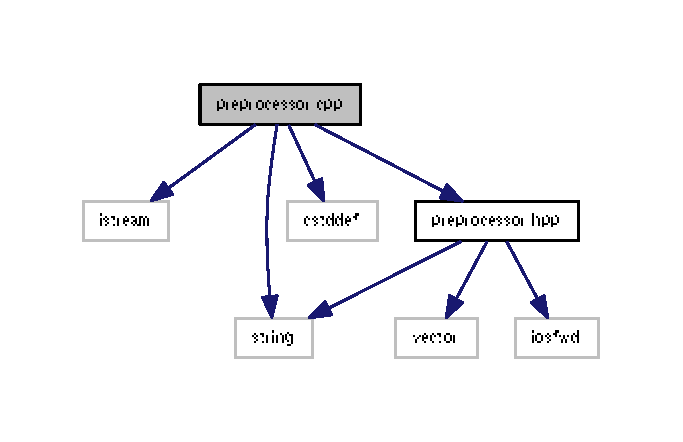
\includegraphics[width=328pt]{preprocessor_8cpp__incl}
\end{center}
\end{figure}

\hypertarget{preprocessor_8hpp}{}\section{preprocessor.\+hpp File Reference}
\label{preprocessor_8hpp}\index{preprocessor.\+hpp@{preprocessor.\+hpp}}
{\ttfamily \#include $<$string$>$}\\*
{\ttfamily \#include $<$vector$>$}\\*
{\ttfamily \#include $<$iosfwd$>$}\\*
Include dependency graph for preprocessor.\+hpp\+:\nopagebreak
\begin{figure}[H]
\begin{center}
\leavevmode
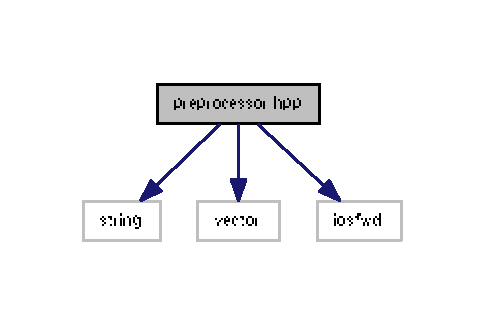
\includegraphics[width=233pt]{preprocessor_8hpp__incl}
\end{center}
\end{figure}
This graph shows which files directly or indirectly include this file\+:
\nopagebreak
\begin{figure}[H]
\begin{center}
\leavevmode
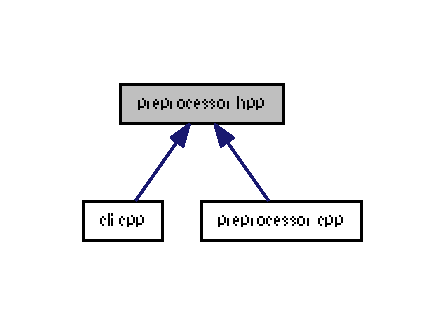
\includegraphics[width=214pt]{preprocessor_8hpp__dep__incl}
\end{center}
\end{figure}
\subsection*{Classes}
\begin{DoxyCompactItemize}
\item 
class \hyperlink{class_scheme_unit}{Scheme\+Unit}
\end{DoxyCompactItemize}

\hypertarget{_r_e_a_d_m_e_8md}{}\section{R\+E\+A\+D\+M\+E.\+md File Reference}
\label{_r_e_a_d_m_e_8md}\index{R\+E\+A\+D\+M\+E.\+md@{R\+E\+A\+D\+M\+E.\+md}}

\hypertarget{biginttest_8cpp}{}\section{test/biginttest.cpp File Reference}
\label{biginttest_8cpp}\index{test/biginttest.\+cpp@{test/biginttest.\+cpp}}
{\ttfamily \#include \char`\"{}utility/bigint.\+hpp\char`\"{}}\\*
{\ttfamily \#include $<$iostream$>$}\\*
{\ttfamily \#include $<$string$>$}\\*
Include dependency graph for biginttest.\+cpp\+:
\nopagebreak
\begin{figure}[H]
\begin{center}
\leavevmode
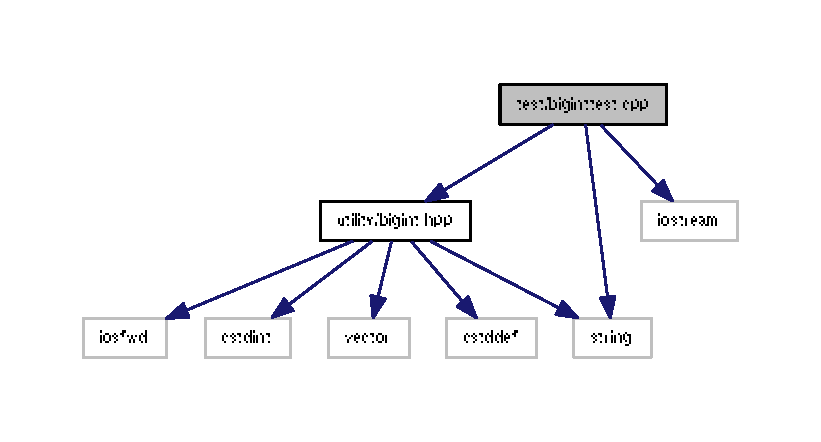
\includegraphics[width=350pt]{biginttest_8cpp__incl}
\end{center}
\end{figure}
\subsection*{Functions}
\begin{DoxyCompactItemize}
\item 
int \hyperlink{biginttest_8cpp_ae66f6b31b5ad750f1fe042a706a4e3d4}{main} ()
\end{DoxyCompactItemize}


\subsection{Function Documentation}
\hypertarget{biginttest_8cpp_ae66f6b31b5ad750f1fe042a706a4e3d4}{}\index{biginttest.\+cpp@{biginttest.\+cpp}!main@{main}}
\index{main@{main}!biginttest.\+cpp@{biginttest.\+cpp}}
\subsubsection[{main}]{\setlength{\rightskip}{0pt plus 5cm}int main (
\begin{DoxyParamCaption}
{}
\end{DoxyParamCaption}
)}\label{biginttest_8cpp_ae66f6b31b5ad750f1fe042a706a4e3d4}


Definition at line 8 of file biginttest.\+cpp.


\hypertarget{preprocessortest_8cpp}{}\section{test/preprocessortest.cpp File Reference}
\label{preprocessortest_8cpp}\index{test/preprocessortest.\+cpp@{test/preprocessortest.\+cpp}}
{\ttfamily \#include \char`\"{}preprocessor.\+hpp\char`\"{}}\\*
{\ttfamily \#include $<$iostream$>$}\\*
{\ttfamily \#include $<$fstream$>$}\\*
Include dependency graph for preprocessortest.\+cpp\+:
\nopagebreak
\begin{figure}[H]
\begin{center}
\leavevmode
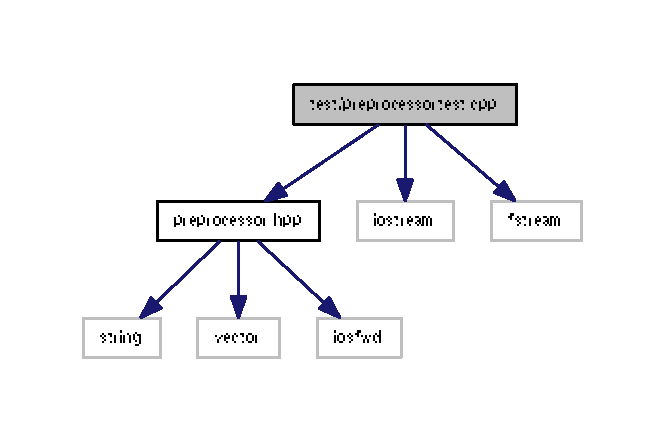
\includegraphics[width=319pt]{preprocessortest_8cpp__incl}
\end{center}
\end{figure}
\subsection*{Functions}
\begin{DoxyCompactItemize}
\item 
ifstream \hyperlink{preprocessortest_8cpp_a777949afad88957e993568613aa2dd3d}{stre} (\char`\"{}preprocessor.\+test\char`\"{})
\item 
int \hyperlink{preprocessortest_8cpp_ae66f6b31b5ad750f1fe042a706a4e3d4}{main} ()
\end{DoxyCompactItemize}
\subsection*{Variables}
\begin{DoxyCompactItemize}
\item 
\hyperlink{class_scheme_unit}{Scheme\+Unit} \hyperlink{preprocessortest_8cpp_a10d1ea193b80aa2128e080646057d11c}{s} (\hyperlink{preprocessortest_8cpp_a777949afad88957e993568613aa2dd3d}{stre})
\end{DoxyCompactItemize}


\subsection{Function Documentation}
\hypertarget{preprocessortest_8cpp_ae66f6b31b5ad750f1fe042a706a4e3d4}{}\index{preprocessortest.\+cpp@{preprocessortest.\+cpp}!main@{main}}
\index{main@{main}!preprocessortest.\+cpp@{preprocessortest.\+cpp}}
\subsubsection[{main}]{\setlength{\rightskip}{0pt plus 5cm}int main (
\begin{DoxyParamCaption}
{}
\end{DoxyParamCaption}
)}\label{preprocessortest_8cpp_ae66f6b31b5ad750f1fe042a706a4e3d4}


Definition at line 7 of file preprocessortest.\+cpp.

\hypertarget{preprocessortest_8cpp_a777949afad88957e993568613aa2dd3d}{}\index{preprocessortest.\+cpp@{preprocessortest.\+cpp}!stre@{stre}}
\index{stre@{stre}!preprocessortest.\+cpp@{preprocessortest.\+cpp}}
\subsubsection[{stre}]{\setlength{\rightskip}{0pt plus 5cm}ifstream stre (
\begin{DoxyParamCaption}
\item[{\char`\"{}preprocessor.\+test\char`\"{}}]{}
\end{DoxyParamCaption}
)}\label{preprocessortest_8cpp_a777949afad88957e993568613aa2dd3d}


\subsection{Variable Documentation}
\hypertarget{preprocessortest_8cpp_a10d1ea193b80aa2128e080646057d11c}{}\index{preprocessortest.\+cpp@{preprocessortest.\+cpp}!s@{s}}
\index{s@{s}!preprocessortest.\+cpp@{preprocessortest.\+cpp}}
\subsubsection[{s}]{\setlength{\rightskip}{0pt plus 5cm}{\bf Scheme\+Unit} s({\bf stre})}\label{preprocessortest_8cpp_a10d1ea193b80aa2128e080646057d11c}

\hypertarget{tokenizertest_8cpp}{}\section{test/tokenizertest.cpp File Reference}
\label{tokenizertest_8cpp}\index{test/tokenizertest.\+cpp@{test/tokenizertest.\+cpp}}
{\ttfamily \#include \char`\"{}preprocessor.\+hpp\char`\"{}}\\*
{\ttfamily \#include \char`\"{}tokenizer.\+hpp\char`\"{}}\\*
{\ttfamily \#include $<$iostream$>$}\\*
{\ttfamily \#include $<$fstream$>$}\\*
{\ttfamily \#include $<$algorithm$>$}\\*
{\ttfamily \#include $<$string$>$}\\*
Include dependency graph for tokenizertest.\+cpp\+:
\nopagebreak
\begin{figure}[H]
\begin{center}
\leavevmode
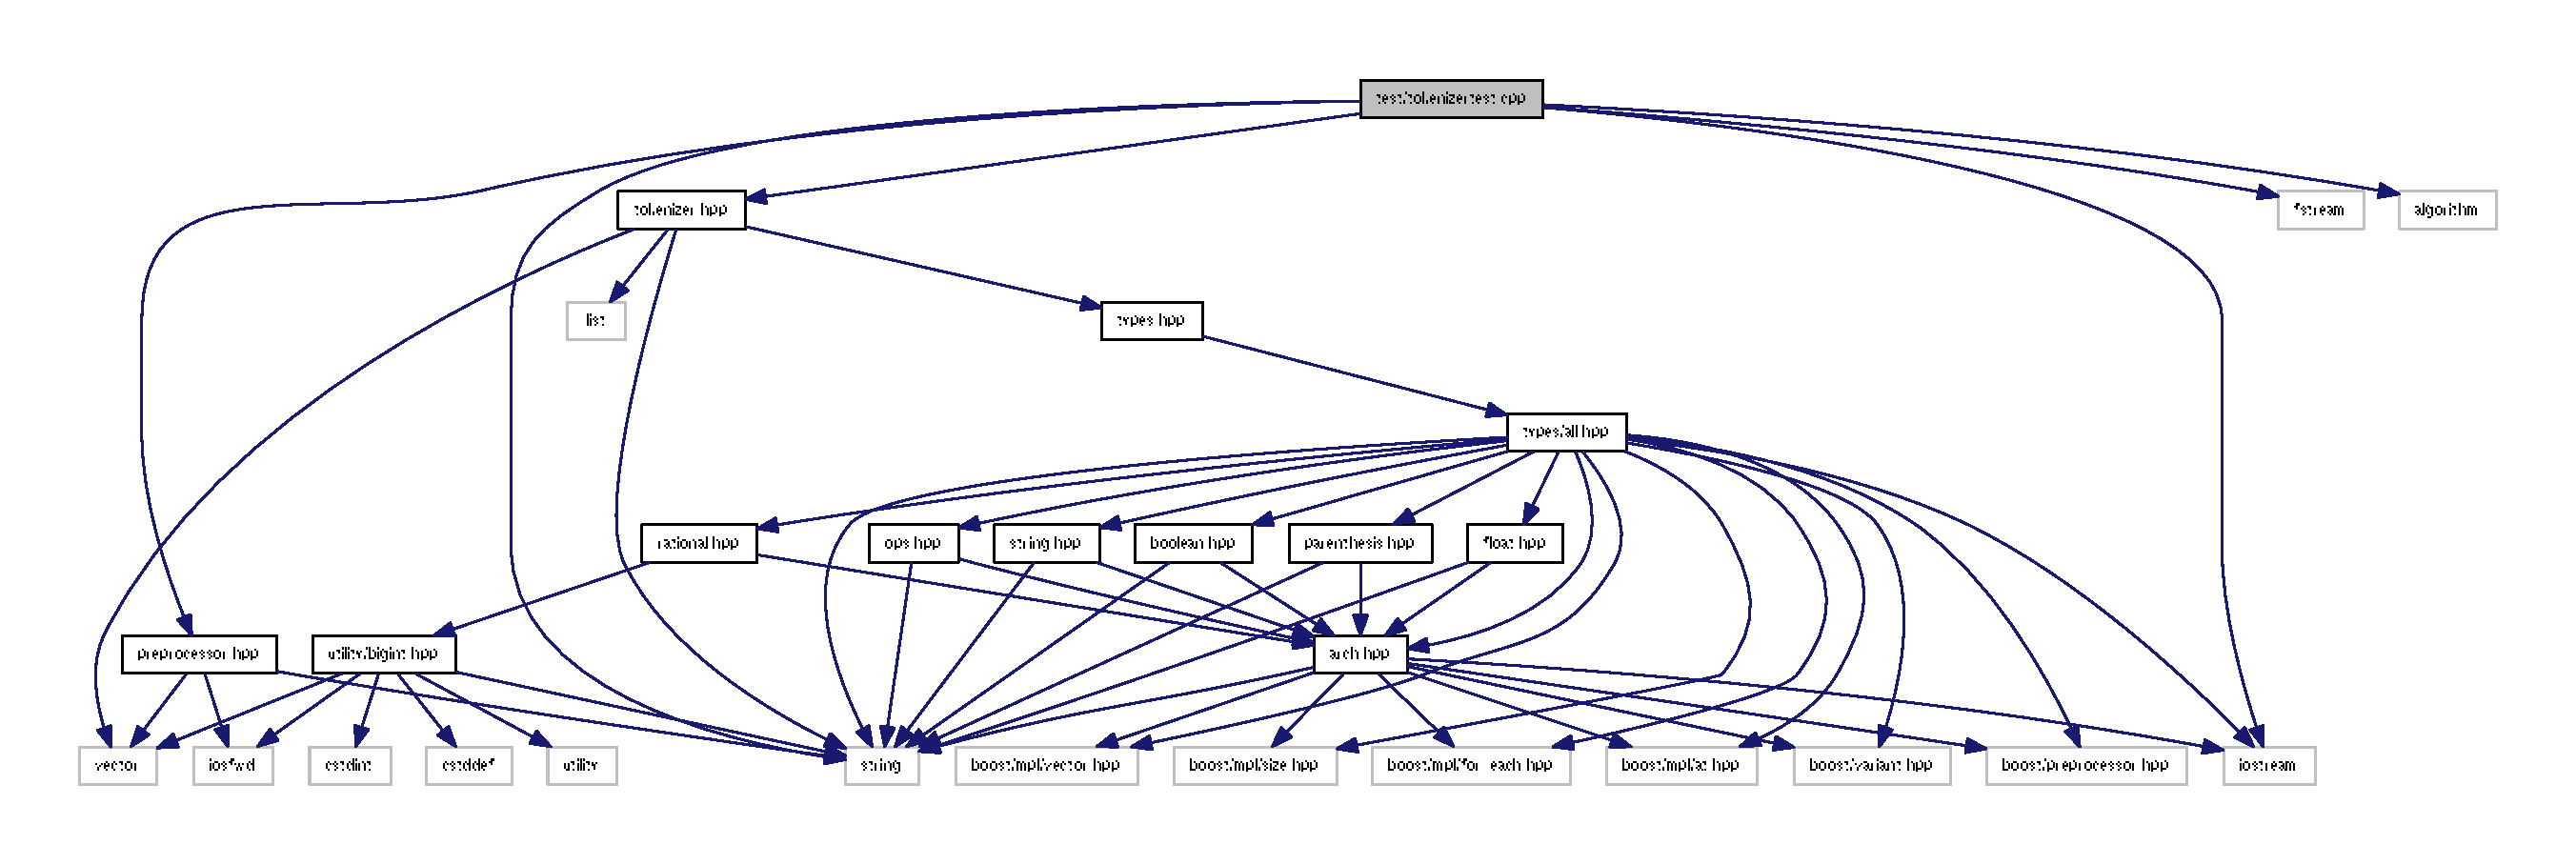
\includegraphics[width=350pt]{tokenizertest_8cpp__incl}
\end{center}
\end{figure}
\subsection*{Functions}
\begin{DoxyCompactItemize}
\item 
int \hyperlink{tokenizertest_8cpp_ae66f6b31b5ad750f1fe042a706a4e3d4}{main} ()
\end{DoxyCompactItemize}


\subsection{Function Documentation}
\hypertarget{tokenizertest_8cpp_ae66f6b31b5ad750f1fe042a706a4e3d4}{}\index{tokenizertest.\+cpp@{tokenizertest.\+cpp}!main@{main}}
\index{main@{main}!tokenizertest.\+cpp@{tokenizertest.\+cpp}}
\subsubsection[{main}]{\setlength{\rightskip}{0pt plus 5cm}int main (
\begin{DoxyParamCaption}
{}
\end{DoxyParamCaption}
)}\label{tokenizertest_8cpp_ae66f6b31b5ad750f1fe042a706a4e3d4}


Definition at line 9 of file tokenizertest.\+cpp.


\hypertarget{tokenizer_8cpp}{}\section{tokenizer.\+cpp File Reference}
\label{tokenizer_8cpp}\index{tokenizer.\+cpp@{tokenizer.\+cpp}}
{\ttfamily \#include \char`\"{}tokenizer.\+hpp\char`\"{}}\\*
{\ttfamily \#include \char`\"{}types.\+hpp\char`\"{}}\\*
{\ttfamily \#include $<$string$>$}\\*
{\ttfamily \#include $<$vector$>$}\\*
{\ttfamily \#include $<$list$>$}\\*
{\ttfamily \#include $<$cstddef$>$}\\*
{\ttfamily \#include $<$algorithm$>$}\\*
{\ttfamily \#include $<$iostream$>$}\\*
Include dependency graph for tokenizer.\+cpp\+:
% FIG 0

\hypertarget{tokenizer_8hpp}{}\section{tokenizer.\+hpp File Reference}
\label{tokenizer_8hpp}\index{tokenizer.\+hpp@{tokenizer.\+hpp}}
{\ttfamily \#include $<$string$>$}\\*
{\ttfamily \#include $<$list$>$}\\*
{\ttfamily \#include $<$vector$>$}\\*
{\ttfamily \#include \char`\"{}types.\+hpp\char`\"{}}\\*
Include dependency graph for tokenizer.\+hpp\+:\nopagebreak
\begin{figure}[H]
\begin{center}
\leavevmode
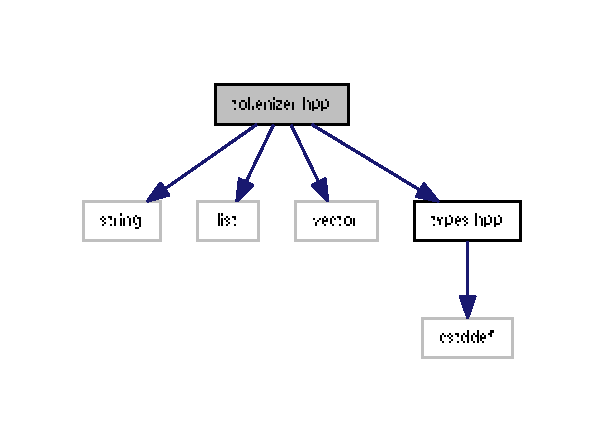
\includegraphics[width=290pt]{tokenizer_8hpp__incl}
\end{center}
\end{figure}
This graph shows which files directly or indirectly include this file\+:\nopagebreak
\begin{figure}[H]
\begin{center}
\leavevmode
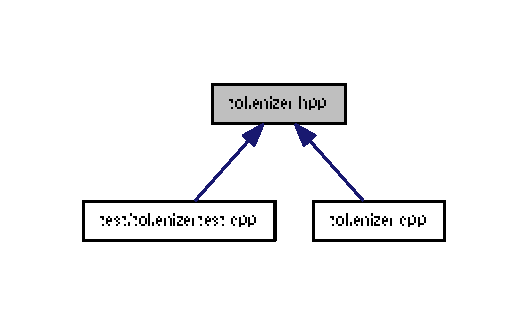
\includegraphics[width=254pt]{tokenizer_8hpp__dep__incl}
\end{center}
\end{figure}
\subsection*{Classes}
\begin{DoxyCompactItemize}
\item 
class \hyperlink{class_tokenizer}{Tokenizer}
\end{DoxyCompactItemize}

\hypertarget{types_8hpp}{}\section{types.\+hpp File Reference}
\label{types_8hpp}\index{types.\+hpp@{types.\+hpp}}
{\ttfamily \#include \char`\"{}types/all.\+hpp\char`\"{}}\\*
Include dependency graph for types.\+hpp\+:
\nopagebreak
\begin{figure}[H]
\begin{center}
\leavevmode
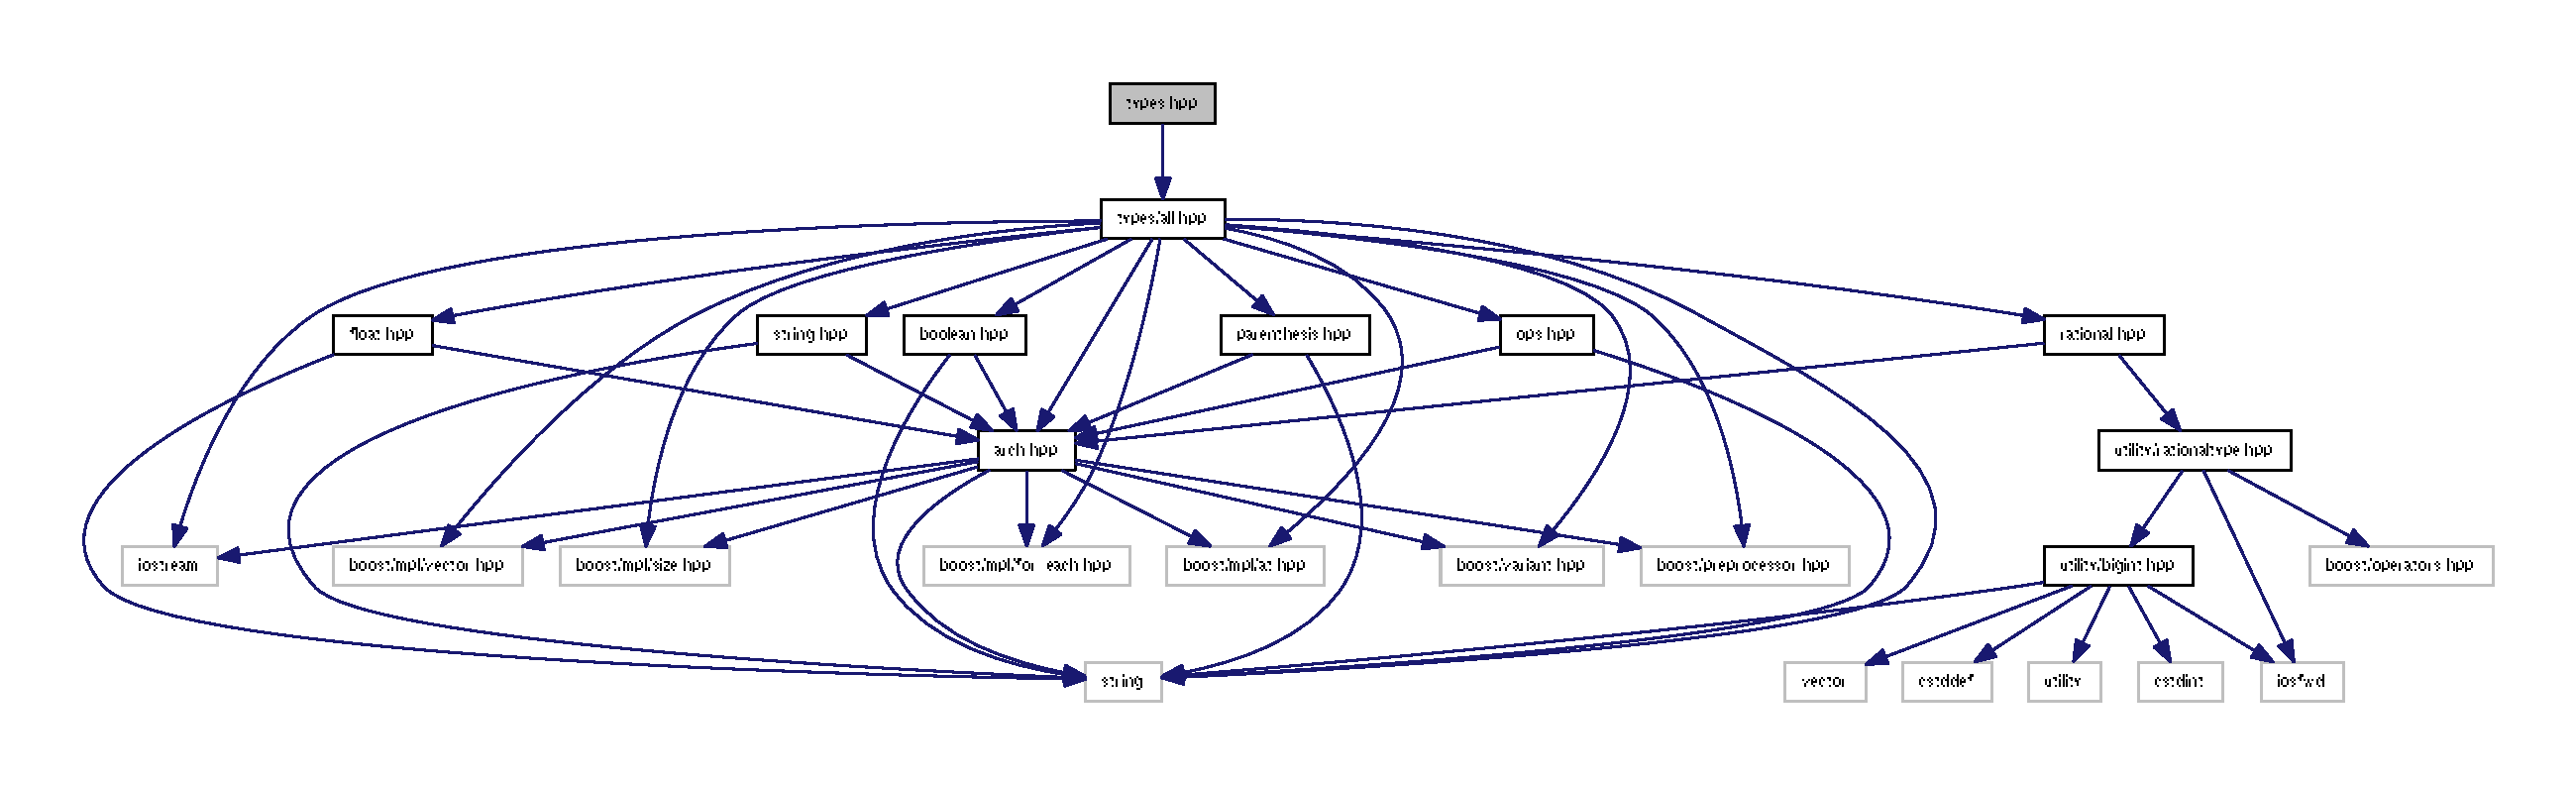
\includegraphics[width=350pt]{types_8hpp__incl}
\end{center}
\end{figure}
This graph shows which files directly or indirectly include this file\+:
\nopagebreak
\begin{figure}[H]
\begin{center}
\leavevmode
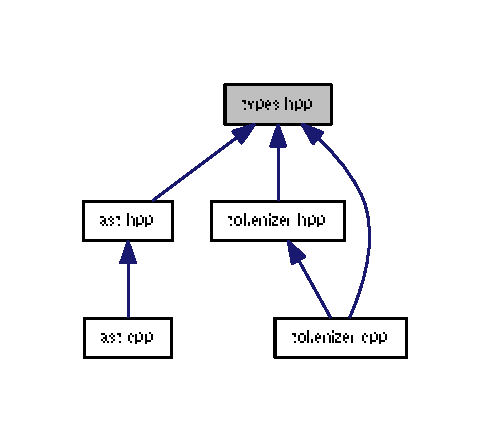
\includegraphics[width=350pt]{types_8hpp__dep__incl}
\end{center}
\end{figure}

\hypertarget{float_8hpp}{}\section{types/float.hpp File Reference}
\label{float_8hpp}\index{types/float.\+hpp@{types/float.\+hpp}}
{\ttfamily \#include \char`\"{}arch.\+hpp\char`\"{}}\\*
{\ttfamily \#include $<$string$>$}\\*
Include dependency graph for float.\+hpp\+:\nopagebreak
\begin{figure}[H]
\begin{center}
\leavevmode
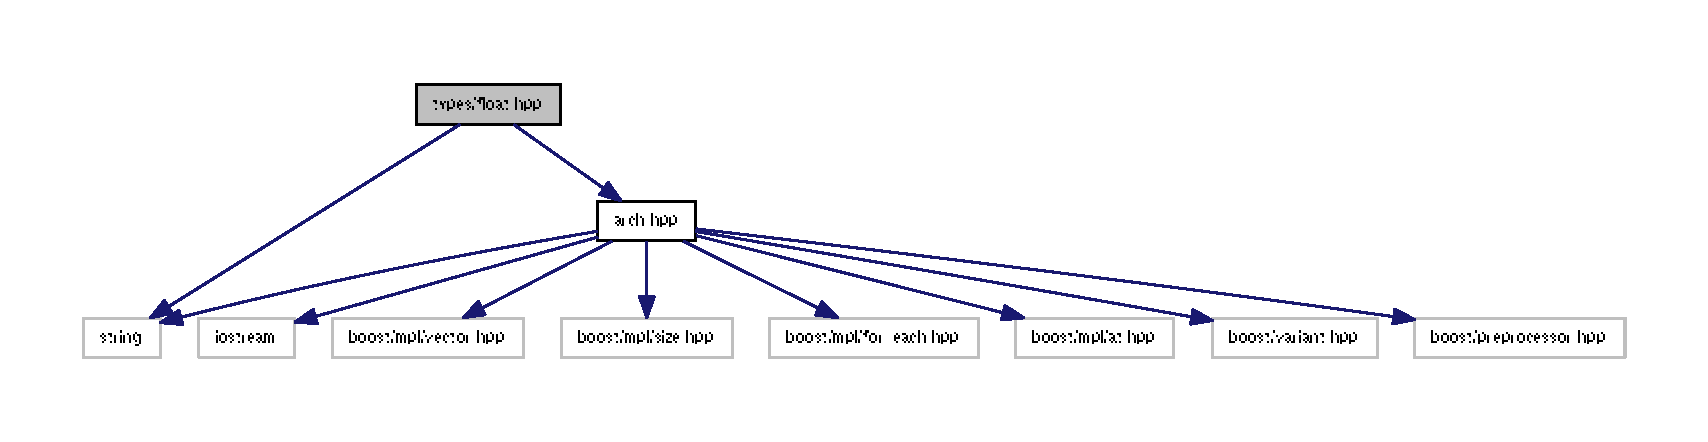
\includegraphics[width=350pt]{float_8hpp__incl}
\end{center}
\end{figure}
This graph shows which files directly or indirectly include this file\+:\nopagebreak
\begin{figure}[H]
\begin{center}
\leavevmode
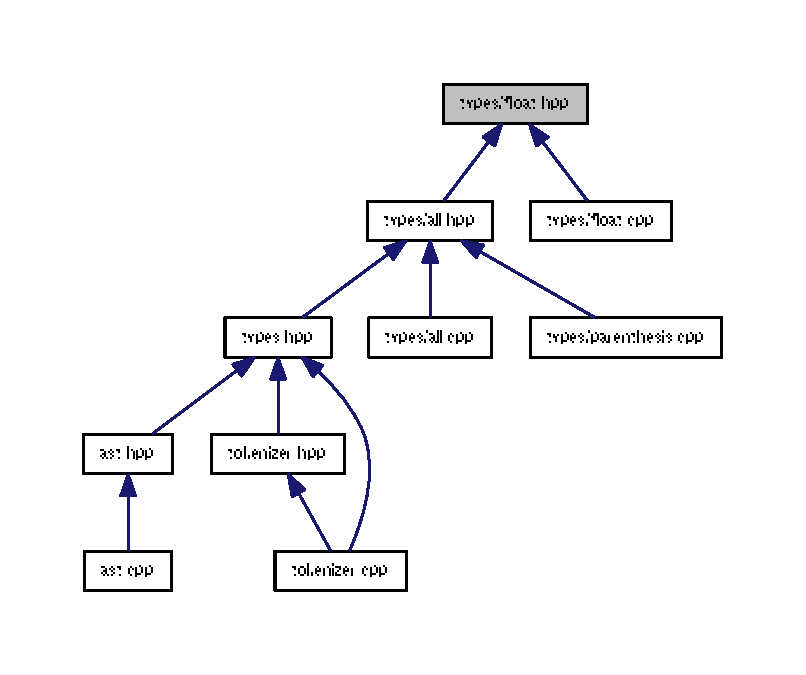
\includegraphics[width=350pt]{float_8hpp__dep__incl}
\end{center}
\end{figure}

\hypertarget{parenthesis_8hpp}{}\section{types/parenthesis.hpp File Reference}
\label{parenthesis_8hpp}\index{types/parenthesis.\+hpp@{types/parenthesis.\+hpp}}
{\ttfamily \#include \char`\"{}arch.\+hpp\char`\"{}}\\*
{\ttfamily \#include $<$string$>$}\\*
Include dependency graph for parenthesis.\+hpp\+:
\nopagebreak
\begin{figure}[H]
\begin{center}
\leavevmode
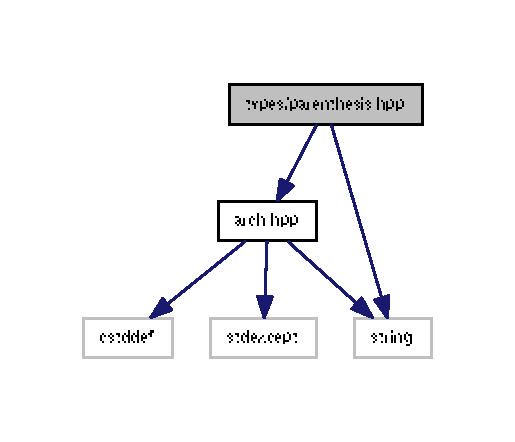
\includegraphics[width=350pt]{parenthesis_8hpp__incl}
\end{center}
\end{figure}
This graph shows which files directly or indirectly include this file\+:
\nopagebreak
\begin{figure}[H]
\begin{center}
\leavevmode
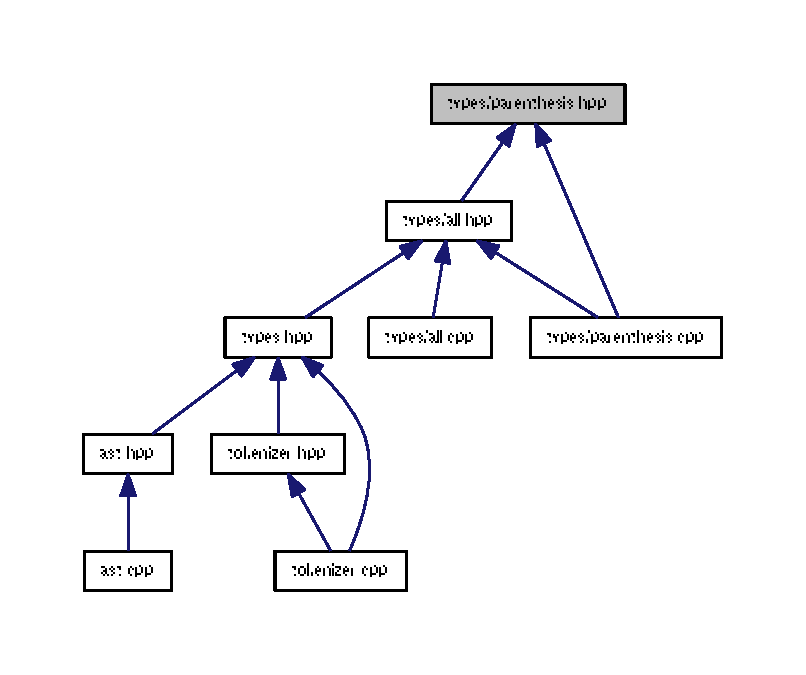
\includegraphics[width=350pt]{parenthesis_8hpp__dep__incl}
\end{center}
\end{figure}

\hypertarget{rational_8hpp}{}\section{types/rational.hpp File Reference}
\label{rational_8hpp}\index{types/rational.\+hpp@{types/rational.\+hpp}}
{\ttfamily \#include \char`\"{}arch.\+hpp\char`\"{}}\\*
{\ttfamily \#include \char`\"{}utility/bigint.\+hpp\char`\"{}}\\*
Include dependency graph for rational.\+hpp\+:\nopagebreak
\begin{figure}[H]
\begin{center}
\leavevmode
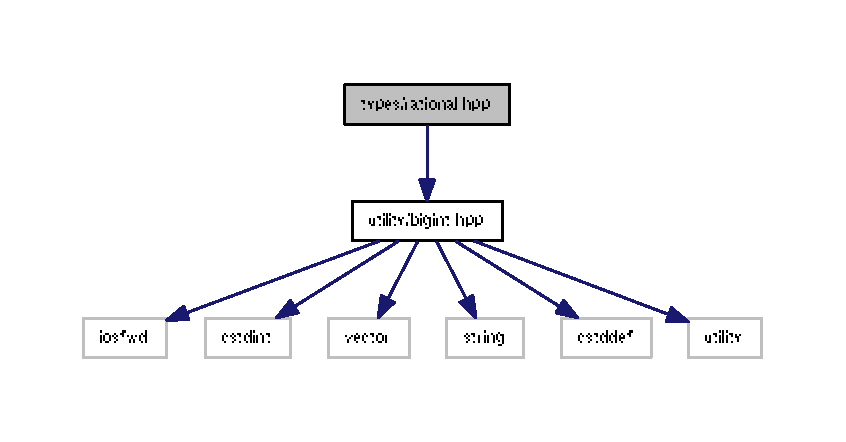
\includegraphics[width=350pt]{rational_8hpp__incl}
\end{center}
\end{figure}
This graph shows which files directly or indirectly include this file\+:\nopagebreak
\begin{figure}[H]
\begin{center}
\leavevmode
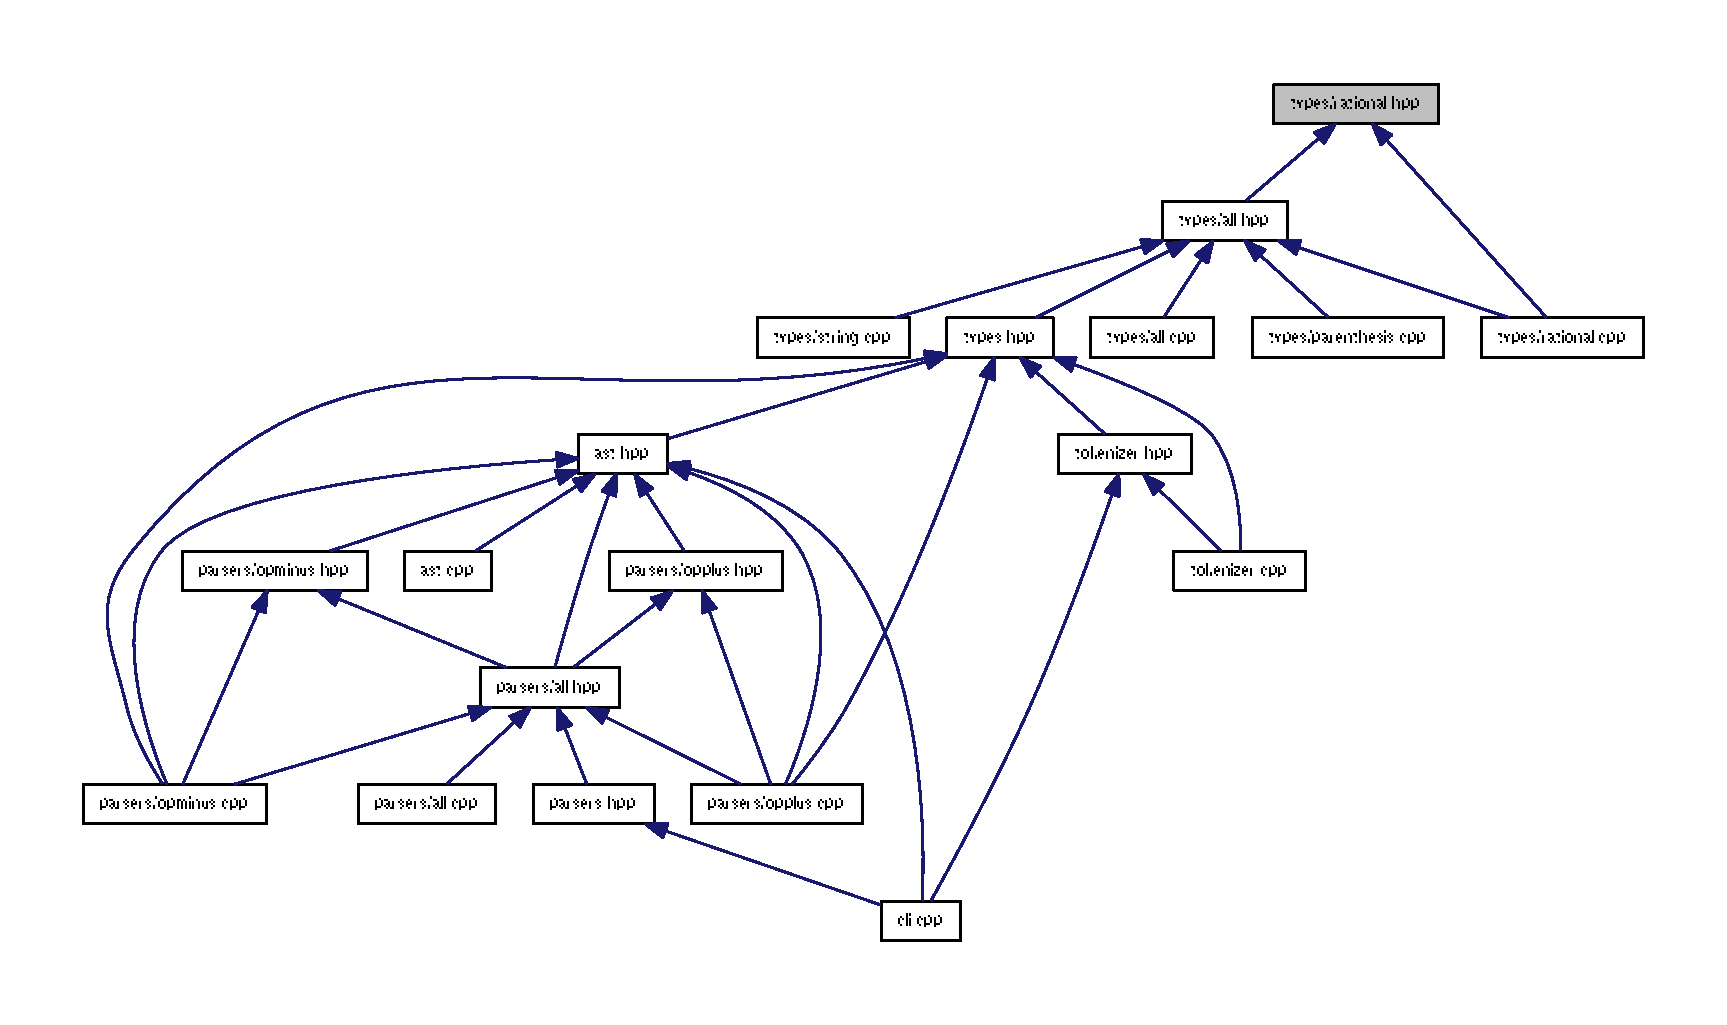
\includegraphics[width=350pt]{rational_8hpp__dep__incl}
\end{center}
\end{figure}
\subsection*{Classes}
\begin{DoxyCompactItemize}
\item 
class \hyperlink{class_rational_type}{Rational\+Type}
\end{DoxyCompactItemize}

\hypertarget{bigint_8cpp}{}\section{utility/bigint.cpp File Reference}
\label{bigint_8cpp}\index{utility/bigint.\+cpp@{utility/bigint.\+cpp}}
{\ttfamily \#include $<$iostream$>$}\\*
{\ttfamily \#include $<$cstdint$>$}\\*
{\ttfamily \#include $<$cstddef$>$}\\*
{\ttfamily \#include $<$vector$>$}\\*
{\ttfamily \#include $<$string$>$}\\*
{\ttfamily \#include $<$cmath$>$}\\*
{\ttfamily \#include $<$cctype$>$}\\*
{\ttfamily \#include $<$stdexcept$>$}\\*
{\ttfamily \#include $<$cassert$>$}\\*
{\ttfamily \#include $<$algorithm$>$}\\*
{\ttfamily \#include $<$utility$>$}\\*
{\ttfamily \#include $<$functional$>$}\\*
{\ttfamily \#include \char`\"{}bigint.\+hpp\char`\"{}}\\*
{\ttfamily \#include \char`\"{}utility/strutility.\+hpp\char`\"{}}\\*
Include dependency graph for bigint.\+cpp\+:\nopagebreak
\begin{figure}[H]
\begin{center}
\leavevmode
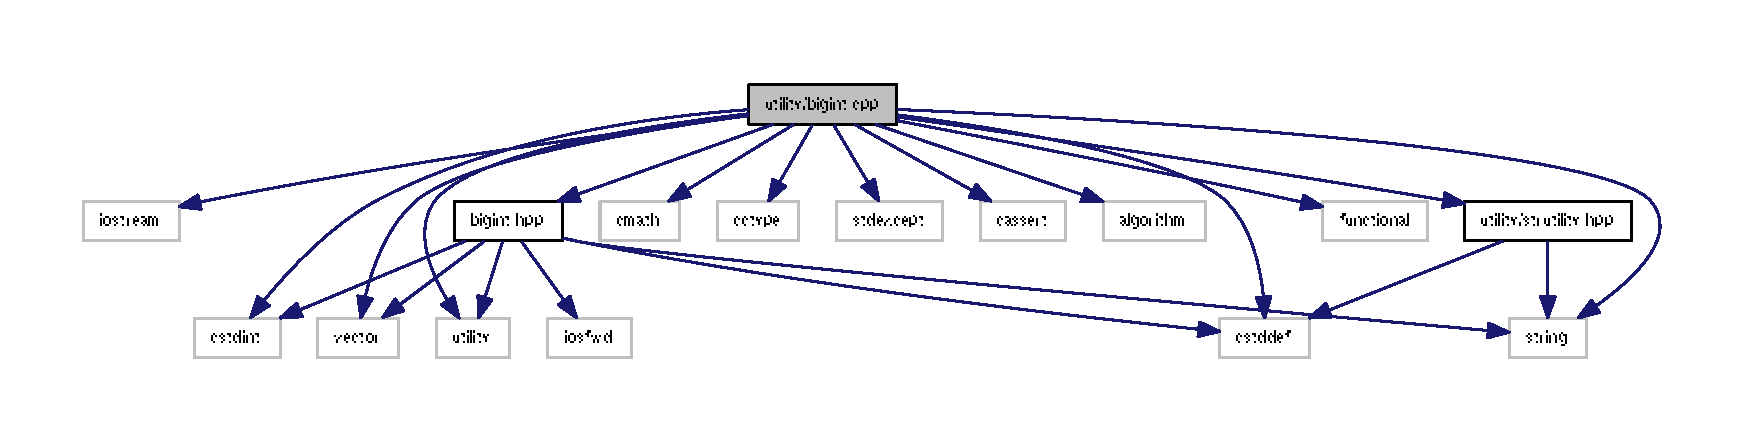
\includegraphics[width=350pt]{bigint_8cpp__incl}
\end{center}
\end{figure}
\subsection*{Functions}
\begin{DoxyCompactItemize}
\item 
{\footnotesize template$<$typename Compare\+Func $>$ }\\bool \hyperlink{bigint_8cpp_a95ccae99f465fac11bf28196f62dac03}{raw\+Compare} (const \hyperlink{class_big_int}{Big\+Int} \&a, const \hyperlink{class_big_int}{Big\+Int} \&b)
\item 
std\+::istream \& \hyperlink{bigint_8cpp_abfb3d978331870b4cba82ece17354f44}{operator$>$$>$} (std\+::istream \&i, \hyperlink{class_big_int}{Big\+Int} \&b)
\item 
std\+::ostream \& \hyperlink{bigint_8cpp_a0d8814d1177634c5e0ee08e2bbccf328}{operator$<$$<$} (std\+::ostream \&o, const \hyperlink{class_big_int}{Big\+Int} \&b)
\end{DoxyCompactItemize}


\subsection{Function Documentation}
\hypertarget{bigint_8cpp_a0d8814d1177634c5e0ee08e2bbccf328}{}\index{bigint.\+cpp@{bigint.\+cpp}!operator$<$$<$@{operator$<$$<$}}
\index{operator$<$$<$@{operator$<$$<$}!bigint.\+cpp@{bigint.\+cpp}}
\subsubsection[{operator$<$$<$}]{\setlength{\rightskip}{0pt plus 5cm}std\+::ostream\& operator$<$$<$ (
\begin{DoxyParamCaption}
\item[{std\+::ostream \&}]{o, }
\item[{const {\bf Big\+Int} \&}]{b}
\end{DoxyParamCaption}
)}\label{bigint_8cpp_a0d8814d1177634c5e0ee08e2bbccf328}


Definition at line 248 of file bigint.\+cpp.

\hypertarget{bigint_8cpp_abfb3d978331870b4cba82ece17354f44}{}\index{bigint.\+cpp@{bigint.\+cpp}!operator$>$$>$@{operator$>$$>$}}
\index{operator$>$$>$@{operator$>$$>$}!bigint.\+cpp@{bigint.\+cpp}}
\subsubsection[{operator$>$$>$}]{\setlength{\rightskip}{0pt plus 5cm}std\+::istream\& operator$>$$>$ (
\begin{DoxyParamCaption}
\item[{std\+::istream \&}]{i, }
\item[{{\bf Big\+Int} \&}]{b}
\end{DoxyParamCaption}
)}\label{bigint_8cpp_abfb3d978331870b4cba82ece17354f44}


Definition at line 240 of file bigint.\+cpp.

\hypertarget{bigint_8cpp_a95ccae99f465fac11bf28196f62dac03}{}\index{bigint.\+cpp@{bigint.\+cpp}!raw\+Compare@{raw\+Compare}}
\index{raw\+Compare@{raw\+Compare}!bigint.\+cpp@{bigint.\+cpp}}
\subsubsection[{raw\+Compare}]{\setlength{\rightskip}{0pt plus 5cm}template$<$typename Compare\+Func $>$ bool raw\+Compare (
\begin{DoxyParamCaption}
\item[{const {\bf Big\+Int} \&}]{a, }
\item[{const {\bf Big\+Int} \&}]{b}
\end{DoxyParamCaption}
)}\label{bigint_8cpp_a95ccae99f465fac11bf28196f62dac03}


Definition at line 104 of file bigint.\+cpp.


\hypertarget{bigint_8hpp}{}\section{utility/bigint.hpp File Reference}
\label{bigint_8hpp}\index{utility/bigint.\+hpp@{utility/bigint.\+hpp}}
{\ttfamily \#include $<$iosfwd$>$}\\*
{\ttfamily \#include $<$cstdint$>$}\\*
{\ttfamily \#include $<$vector$>$}\\*
{\ttfamily \#include $<$string$>$}\\*
{\ttfamily \#include $<$cstddef$>$}\\*
Include dependency graph for bigint.\+hpp\+:
% FIG 0
This graph shows which files directly or indirectly include this file\+:
% FIG 1
\subsection*{Classes}
\begin{DoxyCompactItemize}
\item 
class \hyperlink{class_big_int}{Big\+Int}
\end{DoxyCompactItemize}

\hypertarget{strutility_8hpp}{}\section{utility/strutility.hpp File Reference}
\label{strutility_8hpp}\index{utility/strutility.\+hpp@{utility/strutility.\+hpp}}
{\ttfamily \#include $<$string$>$}\\*
{\ttfamily \#include $<$cstddef$>$}\\*
Include dependency graph for strutility.\+hpp\+:\nopagebreak
\begin{figure}[H]
\begin{center}
\leavevmode
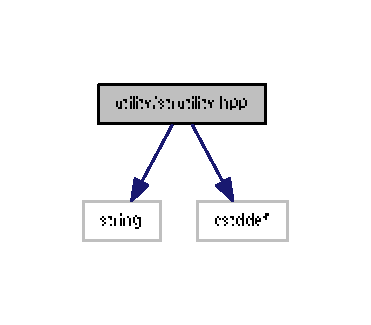
\includegraphics[width=178pt]{strutility_8hpp__incl}
\end{center}
\end{figure}
This graph shows which files directly or indirectly include this file\+:\nopagebreak
\begin{figure}[H]
\begin{center}
\leavevmode
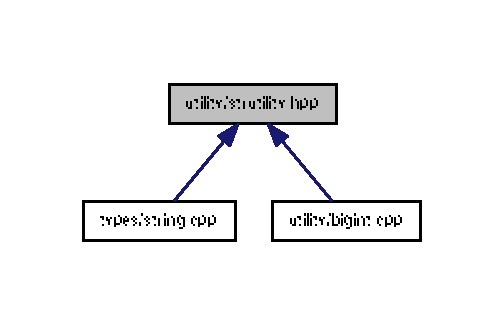
\includegraphics[width=160pt]{strutility_8hpp__dep__incl}
\end{center}
\end{figure}
\subsection*{Functions}
\begin{DoxyCompactItemize}
\item 
bool \hyperlink{strutility_8hpp_a69acba17610caf72f77c862708f34368}{not\+Special\+Char} (const std\+::string \&s, size\+\_\+t pos)
\item 
bool \hyperlink{strutility_8hpp_ae25c1abd5f5eaf0f14c30e568634d19b}{is\+Char} (const std\+::string \&s, size\+\_\+t pos, char c)
\item 
std\+::string \hyperlink{strutility_8hpp_a379b6fa9ecf1c1f18322b4df23d03a09}{char2\+Str} (char c)
\item 
int \hyperlink{strutility_8hpp_aa89ab81c57b043fde24b7660a880efa7}{char2int} (char c)
\end{DoxyCompactItemize}


\subsection{Function Documentation}
\hypertarget{strutility_8hpp_aa89ab81c57b043fde24b7660a880efa7}{}\index{strutility.\+hpp@{strutility.\+hpp}!char2int@{char2int}}
\index{char2int@{char2int}!strutility.\+hpp@{strutility.\+hpp}}
\subsubsection[{char2int}]{\setlength{\rightskip}{0pt plus 5cm}int char2int (
\begin{DoxyParamCaption}
\item[{char}]{c}
\end{DoxyParamCaption}
)\hspace{0.3cm}{\ttfamily [inline]}}\label{strutility_8hpp_aa89ab81c57b043fde24b7660a880efa7}


Definition at line 8 of file strutility.\+hpp.

\hypertarget{strutility_8hpp_a379b6fa9ecf1c1f18322b4df23d03a09}{}\index{strutility.\+hpp@{strutility.\+hpp}!char2\+Str@{char2\+Str}}
\index{char2\+Str@{char2\+Str}!strutility.\+hpp@{strutility.\+hpp}}
\subsubsection[{char2\+Str}]{\setlength{\rightskip}{0pt plus 5cm}std\+::string char2\+Str (
\begin{DoxyParamCaption}
\item[{char}]{c}
\end{DoxyParamCaption}
)\hspace{0.3cm}{\ttfamily [inline]}}\label{strutility_8hpp_a379b6fa9ecf1c1f18322b4df23d03a09}


Definition at line 7 of file strutility.\+hpp.

\hypertarget{strutility_8hpp_ae25c1abd5f5eaf0f14c30e568634d19b}{}\index{strutility.\+hpp@{strutility.\+hpp}!is\+Char@{is\+Char}}
\index{is\+Char@{is\+Char}!strutility.\+hpp@{strutility.\+hpp}}
\subsubsection[{is\+Char}]{\setlength{\rightskip}{0pt plus 5cm}bool is\+Char (
\begin{DoxyParamCaption}
\item[{const std\+::string \&}]{s, }
\item[{size\+\_\+t}]{pos, }
\item[{char}]{c}
\end{DoxyParamCaption}
)\hspace{0.3cm}{\ttfamily [inline]}}\label{strutility_8hpp_ae25c1abd5f5eaf0f14c30e568634d19b}


Definition at line 6 of file strutility.\+hpp.

\hypertarget{strutility_8hpp_a69acba17610caf72f77c862708f34368}{}\index{strutility.\+hpp@{strutility.\+hpp}!not\+Special\+Char@{not\+Special\+Char}}
\index{not\+Special\+Char@{not\+Special\+Char}!strutility.\+hpp@{strutility.\+hpp}}
\subsubsection[{not\+Special\+Char}]{\setlength{\rightskip}{0pt plus 5cm}bool not\+Special\+Char (
\begin{DoxyParamCaption}
\item[{const std\+::string \&}]{s, }
\item[{size\+\_\+t}]{pos}
\end{DoxyParamCaption}
)\hspace{0.3cm}{\ttfamily [inline]}}\label{strutility_8hpp_a69acba17610caf72f77c862708f34368}


Definition at line 5 of file strutility.\+hpp.


%--- End generated contents ---

% Index
\backmatter
\newpage
\phantomsection
\clearemptydoublepage
\addcontentsline{toc}{chapter}{Index}
\printindex

\end{document}
